% =====================================================================
% Научно-исследовательская работа (НИР)
% СПбГУ, факультет ПМ-ПУ, БД116
% Тема: Механистический анализ расхождения KV-кэша при FP8/HQQ-
%       квантизации в reasoning-моделях. Защитные рецепты и прогноз
%       точки первого расхождения через 1D-CNN на K-матрицах.
% Компилировать: pdflatex nir_report.tex (дважды для toc)
% =====================================================================
\documentclass[a4paper,12pt]{article}

\usepackage[T2A]{fontenc}
\usepackage[utf8]{inputenc}
\usepackage[russian]{babel}
\usepackage{geometry}
\geometry{a4paper, left=30mm, right=15mm, top=20mm, bottom=20mm}

\usepackage{graphicx}
\usepackage{booktabs}
\usepackage{amsmath, amssymb}
\usepackage{caption}
\usepackage{float}
\usepackage{xcolor}
\usepackage{hyperref}
\usepackage{enumitem}
\usepackage{url}
\usepackage{tabularx}
\usepackage{array}

\hypersetup{
  colorlinks=true,
  linkcolor=black,
  citecolor=black,
  urlcolor=blue
}

\renewcommand{\baselinestretch}{1.5}
\setlength{\parindent}{1.25cm}
\graphicspath{{./}{figures/}{../../outputs/}}

\begin{document}

% =====================================================================
% Титул
% =====================================================================
\begin{titlepage}
\centering
\vspace*{1cm}
{\large Санкт-Петербургский государственный университет\par}
{\large Факультет прикладной математики — процессов управления\par}
\vspace{4cm}

{\Large \textbf{ОТЧЁТ}\par}
{\large по научно-исследовательской работе\par}
\vspace{1cm}
{\large на тему:\par}
\vspace{0.5cm}
{\LARGE \textbf{Механистический анализ расхождения KV-кэша при
FP8/HQQ-квантизации в reasoning-моделях. Защитные рецепты и прогноз
точки первого расхождения через 1D-CNN на K-матрицах}\par}

\vspace{3cm}
\begin{flushright}
\begin{tabular}{rl}
Выполнил: & студент группы БД116 \\
          & Шарабарин Михаил \\[0.5cm]
Научный руководитель: & Дик Александр Геннадьевич \\
\end{tabular}
\end{flushright}

\vfill
{\large Санкт-Петербург\par}
{\large 2026\par}
\end{titlepage}

\tableofcontents
\newpage

% =====================================================================
% АННОТАЦИЯ (что было сделано и что вышло — на одной странице)
% =====================================================================
\section*{Аннотация}
\addcontentsline{toc}{section}{Аннотация}

\textbf{Что решает работа.} В современных reasoning-моделях (Qwen3,
DeepSeek-R1, OpenAI o1) основной ресурс во время инференса --- KV-кэш
(хранилище ключей и значений механизма attention). Чтобы экономить
память, его квантизуют в FP8 или INT4/INT2 (HQQ). Существующая
литература описывает эффект только агрегированно («accuracy упала на
$N$\%») и не объясняет \textit{механизм}: где именно в модели возникает
шум, как он распространяется и при каком условии токен-поток ломается.
В данной работе мы строим количественную mechanistic chain «шум $K$
$\to$ сдвиг attention $\to$ дрейф hidden $\to$ ошибка logits $\to$ flip
argmax», тестируем интуитивный защитный рецепт в реальной
production-ситуации и предлагаем ML-метод прогноза точки первого
расхождения (First Divergence Point, FDP).

\textbf{Что было сделано.}
\begin{enumerate}[label=\arabic*.,leftmargin=*]
\item Реализован CPU-pipeline на основе \texttt{transformers}, который
  через monkey-patch textit{внутри}
  forward-прохода захватывает $Q$, $K_\text{pre}/K_\text{post}$,
  $V_\text{pre}/V_\text{post}$ и логиты на всех 28 слоях Qwen3-1.7B.
\item На 80 задачах AIME-24 + MATH-500, 4 форматах квантизации и
  2 режимах (teacher-forced + autoregressive) проведено разложение
  шума по (слою, голове, позиции, каналу).
\item Проложена и численно подтверждена цепочка расхождения. Найден
  главный архитектурный артефакт FP8: \textbf{10 каналов из 1024 (1\%)
  концентрируют 51,7\% всего K-шума на Qwen3-1.7B}; HQQ за счёт
  per-group scale размазывает шум в 4--5 раз более равномерно.
\item Проверен защитный рецепт «защитить top-10 каналов в bf16»: в
  лабораторной teacher-forced метрике он восстанавливает 34\% K-ошибки,
  \textbf{но в реальной авторегрессивной генерации эффект исчезает} (-2,4\%
  logit KL, аргмакс начинает флипать с \textasciitilde 40-го шага).
\item Кросс-семейная валидация на 4 моделях (Qwen3-1.7B, Qwen2.5-1.5B,
  SmolLM2-1.7B, DeepSeek-R1-Distill-Qwen-1.5B) показала: цифра 51,7\% ---
  свойство конкретно Qwen3-1.7B, на SmolLM2 (Llama-arch) концентрация
  всего 17\% и рецепт почти не работает. \textbf{Найдена количественная
  межсемейная зависимость:}
  \(\text{recovery} \approx 0{,}65 \cdot \text{top10\_fraction}\) ---
  линейный закон, связывающий концентрацию шума с эффективностью защиты,
  устойчивый на всех 4 архитектурах.
\item Обучен 1D-CNN на K-матрицах, предсказывающий FDP. На 5-fold
  cross-validation $R^2 = 0{,}98$, но на out-of-distribution-задачах
  (где модель отвечает качественно и длинно) R² падает: модель считает
  такие ответы выбросами и плохо предсказывает их FDP. Задача
  переформулирована как ranking (Spearman $\rho = 0{,}70$ на свежих
  задачах) — этого достаточно для production-применения.
\end{enumerate}

\textbf{Главные фундаментально новые результаты} (то, ради чего
писалась эта НИР):

\begin{enumerate}[label=\textbf{Ф.\arabic*.},leftmargin=1.5cm]
\item \textbf{Количественная mechanistic-цепочка KV-quant расхождения
  построена впервые на per-(слой, голова, позиция, канал) уровне.}
  Каждое из четырёх звеньев («шум $K$ $\to$ softmax-усиление $\to$
  cascade $\to$ flip в точке минимального margin») измерено и
  подтверждено на захваченных тензорах. До нашей работы аналогичной
  per-уровневой декомпозиции в открытых источниках нет.
\item \textbf{Структурный закон ``lab $\to$ production''-разрыва.}
  Защитные рецепты, эффективные в одиночном forward (teacher-forced
  метрика), \textit{систематически переоценивают} свою практическую
  пользу в реальной авторегрессивной генерации. Рецепт, восстанавливающий
  -34\% K-ошибки в TF, даёт лишь -2,4\% logit-KL в AR (в пределах шума).
  Причина структурная (decode-шаг видит лишь один новый K-токен, identity
  outlier-каналов нестабильна между шагами) --- значит, \textbf{любой}
  TF-оценённый рецепт обязан проходить отдельную AR-валидацию.
\item \textbf{Межсемейный закон ``concentration $\to$ recovery''.}
  Эффективность защиты top-$N$ каналов в bf16 линейно зависит от
  концентрации K-шума в этих каналах:
  \(\text{recovery} \approx 0{,}65 \cdot \text{top10\_fraction}\).
  Подтверждено на 4 архитектурно разных моделях. Это даёт инженерам
  простой априорный критерий: измерить top-10 fraction за один прогон
  --- и предсказать пользу защиты до её внедрения.
\end{enumerate}

\textbf{Дополнительные результаты:}
\begin{itemize}[leftmargin=*]
\item Прогноз FDP по K-матрицам в форме ranking-task --- работоспособный
  инструмент для adaptive batching и online canary, если переобучить под
  целевую модель ($\rho = 0{,}70$ на out-of-distribution свежих задачах).
\item FDP --- emergent-свойство декодирования, \textbf{не предсказуемое
  из промпта} (подтверждено на двух архитектурно разных моделях). Это
  закрывает целое направление гипотез про офлайн-классификацию задач
  по хрупкости к квантизации.
\end{itemize}

\newpage

% =====================================================================
% ВВЕДЕНИЕ — даёт roadmap и мотивацию
% =====================================================================
\section{Введение}

\subsection{Почему вообще возникла эта задача}

В Qwen3-1.7B одна задача AIME-24 в reasoning-режиме генерирует
\textasciitilde 1500 токенов рассуждений (Chain-of-Thought). К концу
такой генерации KV-кэш --- два тензора формы $[B, H_{kv}, L_{seq}, d_h]$
на каждом из 28 слоёв --- занимает
$28 \times 8 \times 1500 \times 128 \times 2 \approx 17$~МБ на одну
инстанцию. При batch-е 32 это уже \textasciitilde 540~МБ только под
кэш, и память становится главным узким местом. Поэтому
production-стэки (vLLM, SGLang) по умолчанию переключают KV-кэш в FP8,
получая 2$\times$ экономию памяти «бесплатно».

Но действительно ли бесплатно? Промышленные benchmark-ы говорят
«accuracy практически не упала». Мы хотим понять \textit{что
происходит внутри} модели: почему квантизация \textit{всегда} меняет
поток токенов (как мы покажем в части 3), но \textit{иногда} это
ничего не ломает, а иногда сваливает модель в петлю на первом же
токене.

\subsection{Что уже было сделано в литературе}

Существующая литература закрывает только техническую часть KV-quant:

\begin{itemize}[leftmargin=*]
\item \textbf{Форматы FP8} (Micikevicius~\cite{micikevicius2022}) и
  \textbf{HQQ}~\cite{badri2023} описаны как самостоятельные форматы
  квантизации.
\item \textbf{vLLM}~\cite{kwon2023} --- production-стэк, где KV-quant
  применяется по умолчанию.
\item \textbf{SmoothQuant / AWQ}~\cite{xiao2023smoothquant,lin2024awq}
  --- per-channel scaling, но для квантизации весов, не для KV-кэша.
\end{itemize}

\textbf{Чего нет в литературе и что мы делаем в работе.}
Во-первых, нет per-(слой, голова, позиция, канал) разложения того,
как именно FP8-шум на $K$ доходит до argmax-flip --- литература
останавливается на benchmark-accuracy. Во-вторых, нет проверки того,
переносятся ли защитные рецепты из teacher-forced метрики в реальную
авторегрессивную генерацию. В-третьих, нет ML-предсказателя FDP. Эти
три пробела закрывает наша работа.

\subsection{Что мы будем делать (карта-маршрут отчёта)}

Отчёт построен как «логическая цепочка»:

\begin{enumerate}[label=\textbf{Часть \arabic*:},leftmargin=2cm]
\item \textbf{Феноменология} (что мы видим со стороны): измеряем
  accuracy, позицию FDP и тип ошибок. Узнаём \textit{что эффект
  существует и нетривиальный}, но не понимаем механизм.
\item \textbf{Mechanism}: вскрываем модель и
  численно прокладываем цепочку шум-$K$ $\to$ attention $\to$ hidden
  $\to$ logit $\to$ flip. Находим архитектурный артефакт: концентрация
  шума в 10 каналах.
\item \textbf{Защитный рецепт}: естественная гипотеза «защитим
  outlier-каналы». Проверяем сначала лабораторно (работает!), потом в
  реальной AR-генерации (\textit{не работает}). Анализируем почему.
\item \textbf{Кросс-семейная валидация}: подозрение, что эффекты
  переоценили под одну модель. Прогоняем pipeline на ещё 3 моделях
  --- claim-ы Qwen-specific.
\item \textbf{ML-прогноз FDP}: строим 1D-CNN, который по K-матрицам
  предсказывает где произойдёт FDP. По дороге косвенно подтверждаем
  mechanism-наблюдения и обнаруживаем, что задачу регрессии нужно
  переформулировать как ranking.
\end{enumerate}

% =====================================================================
% ПОСТАНОВКА
% =====================================================================
\section{Постановка задачи}

\subsection{Объект и предмет}

\textbf{Объект.} Reasoning-модели семейства Qwen и DeepSeek в bf16 на
CPU/GPU. Основная модель для глубокого анализа --- Qwen3-1.7B (28 слоёв,
GQA-8). Для кросс-валидации: Qwen3-4B, Qwen2.5-1.5B-Instruct (GQA-2),
SmolLM2-1.7B-Instruct (Llama-3-arch), DeepSeek-R1-Distill-Qwen-1.5B.

\textbf{Предмет.} Структурные характеристики шума FP8 (e4m3, e5m2) и
HQQ (INT4, INT2) квантизации $K$- и $V$-тензоров и его распространение
через softmax и каскад слоёв до flip-а argmax.

\subsection{Цель и задачи}

\textbf{Цель:} получить количественное mechanistic-описание
расхождения KV-кэша при квантизации и проверить пригодные для практики
рецепты защиты и прогноза.

\textbf{Задачи:}
\begin{enumerate}[label=\arabic*.,leftmargin=*]
\item Спроектировать и реализовать CPU pipeline захвата KV-тензоров и
  логитов с реальным применением квантизации внутри forward-прохода.
\item Измерить структуру шума K-квантизации per-(слой, голова, позиция,
  канал) и проследить, как он распространяется до logits.
\item Сформулировать и протестировать защитный рецепт; сопоставить
  результат в лабораторных (teacher-forced) и production
  (autoregressive) условиях.
\item Провести кросс-семейную валидацию (кросс-семейная означает
  разницу, например, между семейством Qwen и DeepSeek), чтобы понять
  какие claim-ы привязаны к одной модели, а какие универсальны.
\item Построить прогнозную модель (boosting + NN) для FDP-точки и
  оценить её пригодность для production-применения.
\end{enumerate}

% =====================================================================
% МЕТОДОЛОГИЯ
% =====================================================================
\section{Методология}

Эта глава описывает \textit{инструменты}, которыми мы пользуемся
дальше. Ккак мы вообще можем заглянуть внутрь работающей
модели?.

\subsection{Pipeline захвата KV}

Чтобы получить $K_\text{pre}$ (до квантизации) и $K_\text{post}$ (после)
\textit{прямо во время} forward-прохода, мы внедряемся в три точки:

\begin{enumerate}[label=\arabic*.,leftmargin=*]
\item \texttt{forward\_hook} на \texttt{q\_proj} — захват $Q$
  post-projection, pre-RoPE.
\item Monkey-patch функции \texttt{apply\_rotary\_pos\_emb} — захват $Q$
  post-RoPE.
\item \textbf{Class-level monkey-patch \texttt{DynamicCache.update}} ---
  перехват $K, V$ \textit{до} их записи в кэш: применяем квант-функцию,
  сохраняем pre- и post-варианты, и кладём в кэш post-вариант, чтобы
  модель реально работала с квантизованным $K$.
\end{enumerate}

Третий патч принципиален. Наивный \texttt{forward\_hook} на
attention-блоке срабатывает \textit{после} того, как attention уже
использовал bf16 $K/V$ --- квантизация в нём приходит слишком поздно и
логиты не меняются. Корректность реализации подтверждена golden-тестом:
первые 10 декод-токенов совпадают с полностью симулированным vLLM
forward-ом на AIME-24 задаче 0 при fp8\_e4m3.

\subsection{Тестируемые форматы квантизации}

\begin{table}[H]
\centering
\caption{Тестируемые форматы квантизации KV-кэша.}
\label{tab:formats}
\begin{tabular}{lll}
\toprule
Формат & Биты & Реализация \\
\midrule
FP8 e4m3 & 8 (4 exp, 3 mant) & PyTorch \texttt{torch.float8\_e4m3fn} (per-tensor scale) \\
FP8 e5m2 & 8 (5 exp, 2 mant) & PyTorch \texttt{torch.float8\_e5m2} \\
HQQ INT4 & 4 & \texttt{hqq.core.quantize.Quantizer}, group\_size=64, axis=0 \\
HQQ INT2 & 2 & то же, n\_bits=2 \\
\bottomrule
\end{tabular}
\end{table}

\subsection{Метрики}

Все измерения сводятся к трём базовым величинам.

\textbf{1. Относительная ошибка квантизации Фробениуса} per (layer, head):
\[
\varepsilon^{(\ell)}_h = \frac{\|K^{(\ell)}_{:,h,:,\text{pre}} - K^{(\ell)}_{:,h,:,\text{post}}\|_F}{\|K^{(\ell)}_{:,h,:,\text{pre}}\|_F}.
\]

\textbf{2. Attention-map KL} per (layer, position):
\[
\mathrm{KL}\!\left(\mathrm{softmax}\!\left(\tfrac{Q^{(\ell)}_t K^{(\ell)\top}_\text{pre}}{\sqrt{d_h}}\right)\;\Big\|\;\mathrm{softmax}\!\left(\tfrac{Q^{(\ell)}_t K^{(\ell)\top}_\text{post}}{\sqrt{d_h}}\right)\right).
\]

\textbf{3. Точка первого расхождения} (First Divergence Point, FDP) ---
наименьшая позиция $t$, в которой
$\mathrm{argmax}(l_t^\text{bf16}) \ne \mathrm{argmax}(l_t^\text{quant})$.

\subsection{Условия эксперимента и hardware}

\begin{itemize}[leftmargin=*]
\item \textbf{Базовая модель:} \texttt{Qwen/Qwen3-1.7B} (HF revision
  \texttt{70d244cc}).
\item \textbf{Датасет:} 30 задач AIME-24 + 50 задач MATH-500 = 80 задач.
\item \textbf{Декодирование:} greedy ($T=0$, детерминированный argmax,
  результат бит-в-бит воспроизводим $\Rightarrow$ FDP однозначен);
  опционально 3 random seeds при $T=0,6$ для оценки дисперсии.
\item \textbf{Окно захвата:} $W = 251$ позиция, центр на FDP.
\end{itemize}

\begin{table}[H]
\centering
\caption{Распределение этапов по hardware.}
\label{tab:hw}
\small
\begin{tabularx}{\textwidth}{p{3.5cm}p{3.5cm}X}
\toprule
Этап & Где вычислялось & Как именно \\
\midrule
Феноменология (часть~3): bf16/quant генерация на 80 задачах
$\times$ 4 моделях $\times$ 4 квантизациях; LLM-судья для классификации
ошибок &
GPU-сервер (NVIDIA A100, vLLM 0.7.3) &
vLLM с \texttt{kv\_cache\_dtype="fp8\_e4m3"}/"\texttt{fp8\_e5m2}"/HQQ;
greedy decoding; max\_tokens=2048; категоризация ошибок --- Anthropic
Claude API на каждую FDP-пару. \\
\midrule
Mechanistic capture (части~4, 5, 6): покадровый захват
$Q/K_\text{pre}/K_\text{post}/$$V_\text{pre}/V_\text{post}/\text{logits}$
на 80 задачах $\times$ 4 квантизациях $\times$ \{TF, AR\} &
CPU локально (AMD Ryzen 5 7640HS, 15{,}2~ГБ ОЗУ) &
PyTorch 2.12 с native FP8 dtypes; monkey-patch \texttt{DynamicCache.update};
окна по 251 позиции; сохранение в \texttt{safetensors};
\textasciitilde 6--8~ч wall-clock на полный прогон. \\
\midrule
Cross-model live (часть~6): валидация на Qwen2.5-1.5B / SmolLM2-1.7B /
DeepSeek-R1-Distill &
CPU локально &
те же скрипты с заменой \texttt{--model}; $n = 5\text{--}20$ задач на модель. \\
\midrule
FDP predictor (часть~7): GBM, MLP, 1D-CNN на 80--224 признаках &
CPU локально &
scikit-learn \texttt{GradientBoostingRegressor} + PyTorch MLP/CNN; 5-fold CV. \\
\midrule
End-to-end test на свежих задачах (часть~7): bf16/fp8 генерация +
capture + предсказание CNN &
CPU локально &
\texttt{model.generate} через transformers; greedy; max 400--1200
токенов. \\
\bottomrule
\end{tabularx}
\end{table}

\paragraph{Итог методологии.} У нас есть инструмент, который умеет
вытащить \textit{любую} промежуточную величину из работающей модели и
гарантирует, что квантизация применяется в нужный момент. Следующие
главы строятся на этом инструменте: сначала смотрим на проблему
снаружи (часть~3), потом залезаем внутрь (часть~4).

\clearpage

% =====================================================================
% ЧАСТЬ 3 — ФЕНОМЕНОЛОГИЯ
% =====================================================================
\section*{Часть~3. Феноменология: что мы видим со стороны}
\addcontentsline{toc}{section}{Часть~3. Феноменология}

\paragraph{Цель главы.} Прежде чем строить mechanistic-анализ, мы
должны убедиться, что эффект (а)~существует, (б)~нетривиальный и
(в)~зависит от модели и формата квантизации. Это «фотография» проблемы
без объяснения причин.

\subsection*{3.1 Accuracy: где квантизация ломает результат}

100\% задач имеют ненулевой FDP при любой квантизации --- то есть
квантизация \textit{всегда} меняет поток токенов. Но \textit{ломает ли
это финальный ответ} в \texttt{\textbackslash boxed\{\}} ---
по-разному для разных моделей.

\begin{figure}[H]
\centering
\includegraphics[width=0.85\textwidth]{../../outputs/paper/accuracy_bars.png}
\caption{Accuracy по парам (модель $\times$ квантизация) на 80 задачах.}
\label{fig:acc}
\end{figure}

Видим резкий контраст: \textbf{Qwen3-1.7B устойчив} (accuracy в пределах
$\pm 2$~п.п.), \textbf{DeepSeek-R1-Distill коллапсирует} с 35--60\% до
0\% на всех квантизациях. Это первый сигнал, что reasoning-distilled
модели качественно отличаются от base instruction-tuned под
квантизацией. Но \textit{почему} --- пока не понятно.

\subsection*{3.2 Где в trace происходит расхождение}

\textit{Trace} (далее по тексту английский термин «trace» соответствует
русскому «последовательность сгенерированных токенов» или «цепочка
авторегрессивной генерации»). Смотрим, в какой относительной позиции
(0~--- начало, 1~--- конец) впервые возникает FDP.

\begin{figure}[H]
\centering
\includegraphics[width=0.85\textwidth]{../../outputs/paper/divergence_position.png}
\caption{Распределение FDP относительно длины trace.}
\label{fig:divpos}
\end{figure}

\begin{table}[H]
\centering
\caption{Позиция FDP относительно длины trace.}
\label{tab:divpos}
\small
\begin{tabular}{llcccc}
\toprule
Model & Quant & median & mean & std \\
\midrule
deepseek-r1-distill-qwen-1.5b & fp8\_e4m3 & \textbf{0,00} & 0,01 & 0,06 \\
deepseek-r1-distill-qwen-1.5b & fp8\_e5m2 & 0,00 & 0,01 & 0,07 \\
qwen3-1.7b & fp8\_e4m3 & \textbf{0,45} & 0,46 & 0,30 \\
qwen3-1.7b & fp8\_e5m2 & 0,42 & 0,43 & 0,31 \\
\bottomrule
\end{tabular}
\end{table}

DeepSeek диверджит в первом же токене в 95\% задач. Qwen3 --- в
районе середины (0,45). Механизм чувствительности явно разный: DeepSeek
ломается сразу, Qwen3 --- накапливает ошибку.

\subsection*{3.3 Какого типа ошибки производит квантизация}

Каждую FDP-точку LLM-судья (Claude) классифицирует в 6-категорийную
таксономию: A~--- алгебраическая ошибка, B~--- арифметическая, C~---
смена стратегии, D~--- галлюцинация, E~--- переключение метода, F~---
повторение / loop.

\begin{table}[H]
\centering
\caption{Нормированное распределение типов ошибок по форматам.}
\label{tab:chi2}
\begin{tabular}{lcccccc}
\toprule
Метод & A & B & C & D & E & \textbf{F (loop)} \\
\midrule
fp8\_e4m3 & 0,04 & 0,02 & 0,15 & 0,13 & 0,10 & \textbf{0,55} \\
fp8\_e5m2 & 0,03 & 0,05 & 0,11 & 0,04 & 0,08 & \textbf{0,68} \\
hqq\_int2 & 0,00 & 0,00 & 0,00 & 0,07 & 0,23 & \textbf{0,70} \\
hqq\_int4 & 0,05 & 0,00 & 0,00 & 0,06 & 0,12 & \textbf{0,76} \\
\bottomrule
\end{tabular}
\end{table}

Критерий $\chi^2 = 66{,}58$, $\text{dof} = 15$, $p = 1{,}8 \cdot 10^{-8}$,
Cramér's $V = 0{,}187$ --- распределения статистически значимо разные.
Доминирующий тип ошибки везде --- \textbf{F (loop)}; чем сильнее
квантизация, тем чаще модель сваливается в повторение. Это важно запомнить:
к этому факту мы вернёмся в части~7, когда будем оценивать bucket-classifier.

\subsection*{3.4 Парадокс: иногда квантизация \textit{помогает}}

В 5 случаях из 160 fp8-прогонов на Qwen3-1.7B квантизация дала
\textit{правильный} ответ, а bf16 baseline --- нет. Квант-шум подтолкнул
модель на более удачную траекторию рассуждения, чем deterministic bf16.
Это означает, что не вся квант-чувствительность вредна --- иногда она
играет роль случайного поиска. Сам по себе этот факт не центральный, но
он усложняет интерпретацию: «эффект квантизации» не сводится к «потеря
качества».

\paragraph{Итог части 3.} Эффект (а)~есть всегда, (б)~зависит от модели
драматически, (в)~почти всегда выражается в loop-ах, (г)~иногда даже
полезен. Снаружи понятно \textit{что} происходит, но непонятно
\textit{почему}. Чтобы получить ответ, в следующей главе мы вскрываем
модель и смотрим на промежуточные тензоры.

\clearpage

% =====================================================================
% ЧАСТЬ 4 — МЕХАНИЗМ
% =====================================================================
\section*{Часть~4. Mechanism: откуда берётся расхождение}
\addcontentsline{toc}{section}{Часть~4. Mechanism}

\paragraph{Цель главы.} Численно проложить цепочку
\textit{шум $K$ $\to$ сдвиг attention $\to$ дрейф hidden $\to$ ошибка
logits $\to$ flip argmax}. Каждый шаг подкреплён захваченными тензорами.

\subsection*{4.1 Откуда стартует шум: структура K-ошибки}

Средняя относительная ошибка Фробениуса $\varepsilon$ показывает,
насколько сильно разные форматы искажают $K$:

\begin{table}[H]
\centering
\caption{Mean и max относительная ошибка $K$ по 80 задачам.}
\label{tab:kerr}
\begin{tabular}{lcc}
\toprule
Формат & Mean $\varepsilon$ & Max (layer $\times$ head) $\varepsilon$ \\
\midrule
fp8\_e4m3 & \textbf{2,65~\%} & 3,50~\% \\
fp8\_e5m2 & 5,25~\% & 7,32~\% \\
hqq\_int4 & 10,3~\% & --- \\
hqq\_int2 & 60,7~\% & --- \\
\bottomrule
\end{tabular}
\end{table}

Видны два структурных соотношения: $2\times$ между FP8 e4m3 и e5m2
(один лишний бит мантиссы) и $\sim 4\times$ переход FP8 $\to$ HQQ INT4.
Где именно эта ошибка распределена по слоям и головам ---
показывает heatmap:

\begin{figure}[H]
\centering
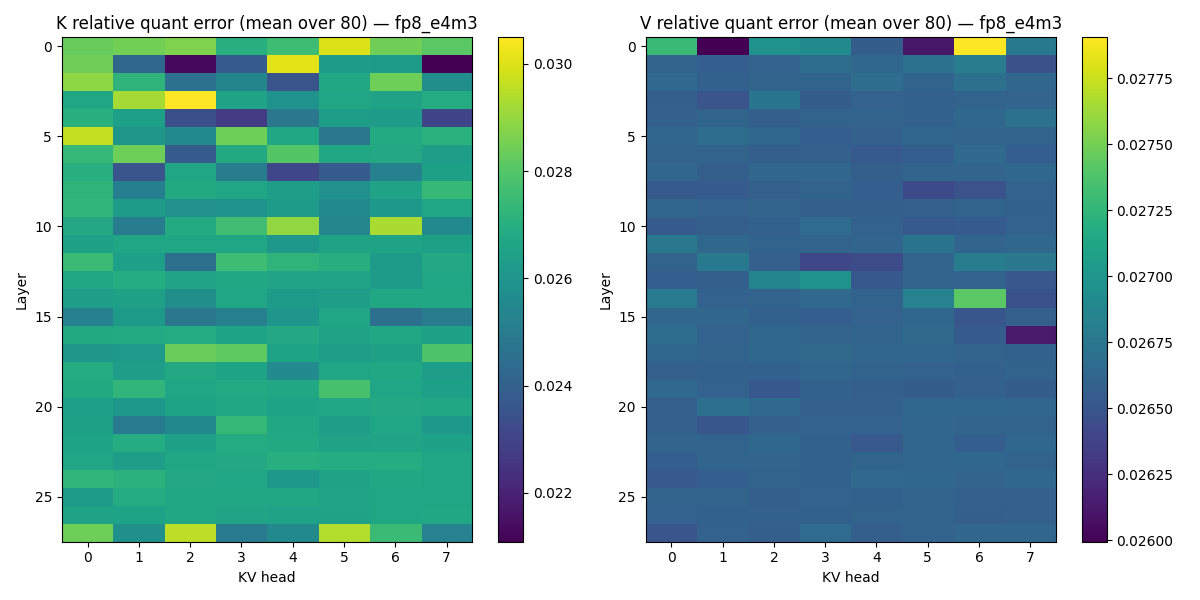
\includegraphics[width=0.85\textwidth]{figures/fig_layer_head.png}
\caption{Heatmap относительной ошибки K-квантизации
$\varepsilon^{(\ell)}_h$ в формате fp8\_e4m3. Слои 0--5 страдают
сильнее.}
\label{fig:layerhead}
\end{figure}

Это уже подсказка, что внутри $K$ что-то распределено неравномерно. На
каком уровне эта неравномерность? Это вопрос следующего раздела.

\subsection*{4.2 Главный артефакт: концентрация шума в каналах}

Для каждого слоя сортируем 1024 канала (8 KV-heads $\times$ 128
head\_dim) по вкладу в $\|K_\text{pre} - K_\text{post}\|_F^2$ и смотрим
кумулятивную долю шума, покрываемую top-$k$ каналами.

\begin{figure}[H]
\centering
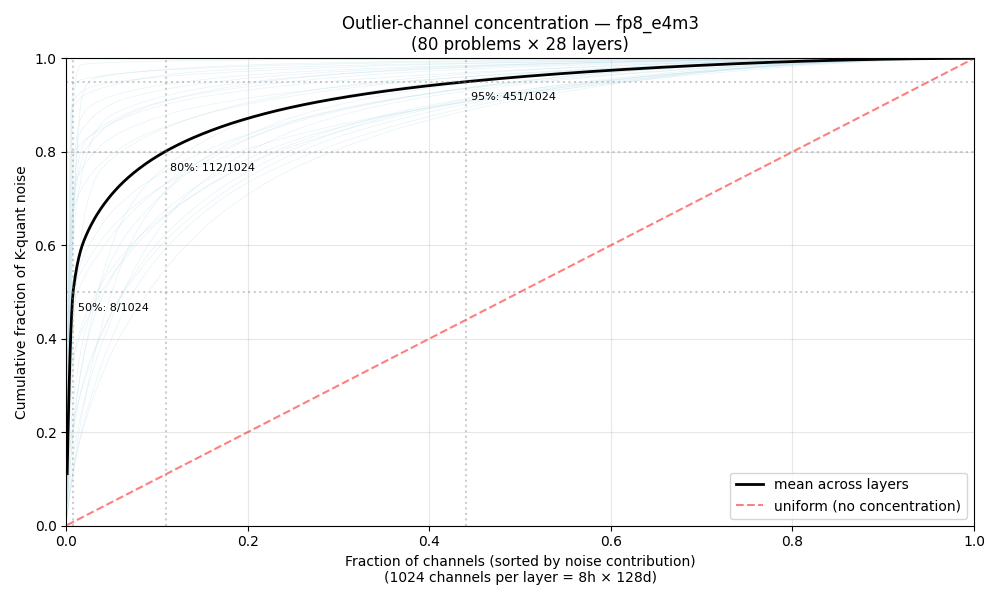
\includegraphics[width=0.82\textwidth]{figures/fig_concentration_fp8.png}
\caption{Кривая концентрации K-шума для fp8\_e4m3 (медиана по 28 слоям
$\times$ 80 задач). \textbf{Top-10 каналов покрывают 51,7\% шума.}}
\label{fig:concfp8}
\end{figure}

\begin{figure}[H]
\centering
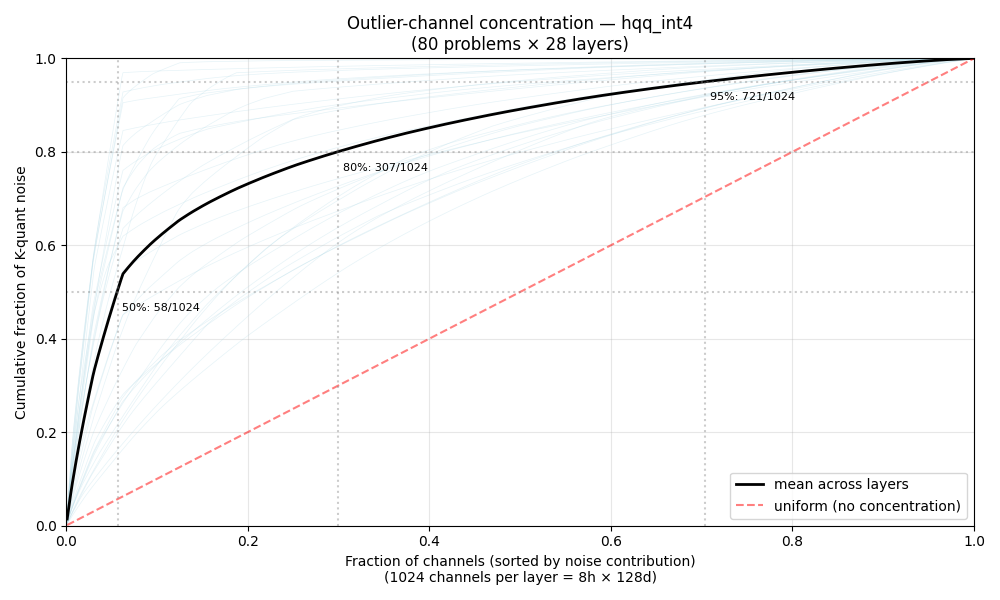
\includegraphics[width=0.82\textwidth]{figures/fig_concentration_hqq.png}
\caption{Та же кривая для hqq\_int4: распределение значительно более
равномерное (top-10 = 13,1\%).}
\label{fig:conchqq}
\end{figure}

\begin{table}[H]
\centering
\caption{Концентрация K-шума: медианы по 28 слоям $\times$ 80 задач.}
\label{tab:conc}
\begin{tabular}{lcccc}
\toprule
Формат & top-1 канал & top-10 & \# ch для 50\% & \# ch для 80\% \\
\midrule
fp8\_e4m3 & \textbf{10,3~\%} & \textbf{51,7~\%} & 8 & 99 \\
fp8\_e5m2 & 10,0~\% & 50,4~\% & 10 & 102 \\
hqq\_int4 & 1,5~\% & 13,1~\% & 53 & 252 \\
hqq\_int2 & 1,6~\% & 14,4~\% & 46 & 251 \\
\bottomrule
\end{tabular}
\end{table}

\textbf{Главное наблюдение.} В FP8 e4m3 одна каналов из 1024 (1\%)
несёт более половины всего шума. Причина в способе квантизации:
\textit{per-tensor} FP8 scale считается по максимуму всего тензора, и
один канал-«выскочка» (outlier) диктует шаг квантизации для всех
остальных. Inlier-каналы при этом теряют точность непропорционально.
HQQ использует \textit{per-group} scale (group\_size = 64) и отдельный
zero-point внутри группы --- поэтому outlier не влияет на соседей, и
распределение шума в \textbf{4 раза равномернее}.

Это не косметическая разница, а структурное свойство, из которого позже
напрямую вытекает гипотеза защитного рецепта (часть~5).

\subsection*{4.3 Outlier-каналы --- свойство весов, а не шума сэмплирования}

Если бы концентрация была артефактом случайного декодирования, при
другом seed-е выделялись бы другие каналы. Проверяем: запускаем 3
независимых seed-а при $T=0{,}6$ и смотрим Jaccard top-10 каналов между
ними.

\textbf{Результат:} медианный Jaccard $= 0{,}879$ (IQR $[0{,}78,\; 1{,}00]$),
концентрация $52{,}5\% \pm 26{,}6\%$. То есть identity outlier-каналов
\textbf{архитектурное свойство выученных весов} модели, не sampling-артефакт.
Это важно: можно один раз снять calibration $K$ и использовать список
outlier-каналов многократно (что мы и попробуем в части~5).

\subsection*{4.4 От K-шума к attention: softmax усиливает в $\sim$100 раз}

Самое интересное происходит при $QK^\top / \sqrt{d_h}$ внутри softmax-а.
Софтмакс --- нелинейный, и небольшая ошибка в $K$ превращается в
большой сдвиг распределения внимания.

\begin{table}[H]
\centering
\caption{Усреднённая по головам attention-KL.}
\label{tab:attnkl}
\begin{tabular}{lcc}
\toprule
Формат & Global mean attn-KL & @FDP \\
\midrule
fp8\_e4m3 & 0,00358 & 0,00352 \\
fp8\_e5m2 & 0,01405 & 0,01334 \\
hqq\_int4 & 0,391   & 0,381   \\
hqq\_int2 & 4,81    & 4,78    \\
\bottomrule
\end{tabular}
\end{table}

Численно: $4\times$ разница в K-ошибке (fp8\_e4m3 $\to$ hqq\_int4)
превращается в $108\times$ разницу в attention-KL ($0{,}00358 \to 0{,}391$).
Это и есть тот самый «усилитель» --- центральный шаг всего механизма.

\subsection*{4.5 От attention к logits: каскад слоёв всё перемешивает}

Естественно ожидать, что слой с самым большим attention-сдвигом будет
давать и самый большой эффект на logits. Проверяем через single-layer
ablation (квантизуем только один слой $\ell$, остальные оставляем
bf16) и сравниваем ranking-и:

\begin{figure}[H]
\centering
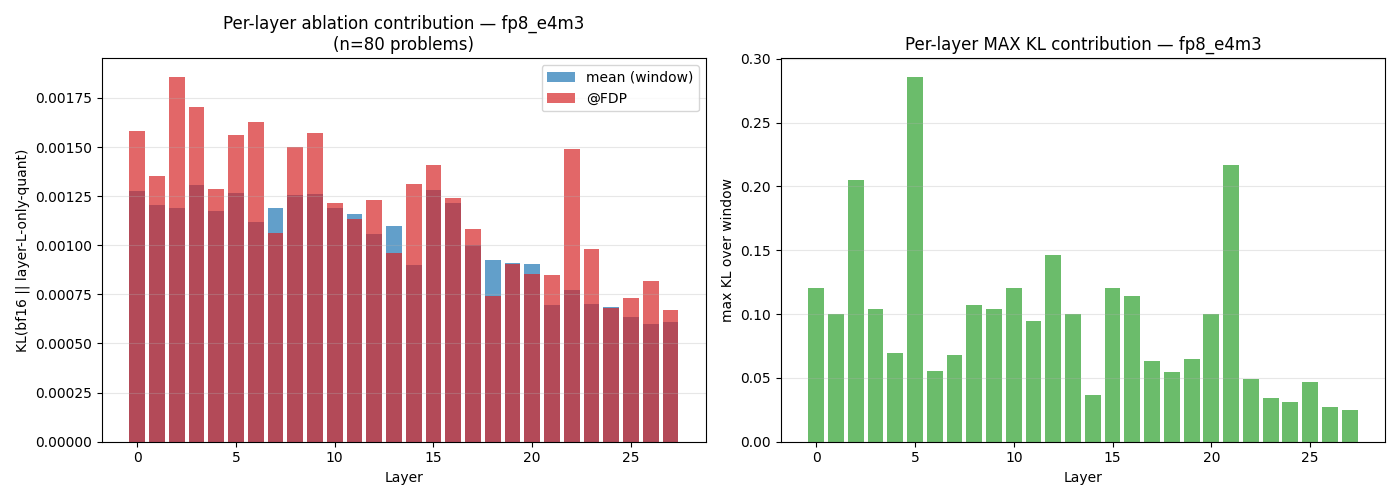
\includegraphics[width=0.85\textwidth]{figures/fig_layer_ablation.png}
\caption{Per-layer logit-impact KL для fp8\_e4m3 при single-layer
ablation.}
\label{fig:layerab}
\end{figure}

\begin{table}[H]
\centering
\caption{Top-5 слоёв по двум метрикам.}
\label{tab:rank}
\begin{tabular}{ccc}
\toprule
Rank & Attention-shift (fp8\_e4m3) & Logit-impact (fp8\_e4m3) \\
\midrule
1 & L5 & L3 \\
2 & L3 & L15 \\
3 & L4 & L0 \\
4 & L13 & L5 \\
5 & L7 & L9 \\
\bottomrule
\end{tabular}
\end{table}

\textit{Ranking-и не совпадают:} L5 --- топ по local attention-shift,
но только 4-й по logit-impact (его шум частично гасится downstream).
L0 наоборот: small local shift, но большой logit-impact, потому что
ошибка \textit{прокатывается} через каскад из 27 последующих слоёв.

Формально:
\[
\operatorname{rank}\!\bigl(\mathrm{KL}_\text{attention}^{(\ell)}\bigr) \;\neq\; \operatorname{rank}\!\bigl(\text{logit-impact}^{(\ell)}\bigr),
\]
где $\operatorname{rank}$ --- упорядочение 28 слоёв по убыванию
соответствующей метрики. Только L3 и L5 входят в top-5 обоих
рейтингов на Qwen3-1.7B. Logit-divergence есть интеграл от
attention-shift по downstream-cascade-глубине, а не точечная величина.

\subsection*{4.6 Когда расходимость взлетает: насыщающаяся экспонента $\tau = 130$}

Если шум прокатывается через каскад, как logit-KL растёт со временем в
AR-режиме? Зависимость хорошо приближается насыщающейся экспонентой:
\[
\mathrm{KL}(t) = K_\infty \bigl(1 - e^{-t/\tau}\bigr).
\]

\begin{figure}[H]
\centering
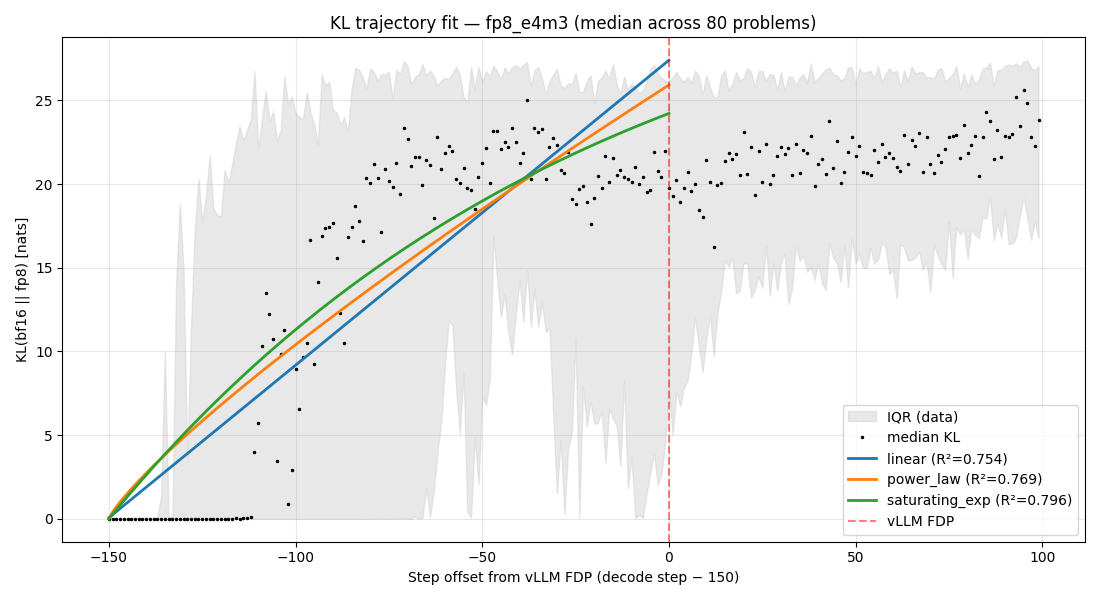
\includegraphics[width=0.85\textwidth]{figures/fig_kl_fit.png}
\caption{Median logit-KL между bf16 и fp8\_e4m3 траекториями в AR-режиме
(80 задач, $T=0$).}
\label{fig:klfit}
\end{figure}

При $T=0$: $\tau = 130$, $R^2 = 0{,}80$. То есть \textbf{первые
$\sim$100--150 токенов} --- активное накопление ошибки. Дальше KL
выходит на плато и траектории уже неотличимы по этой метрике. Это
согласуется с тем, что наблюдаемая median FDP $\approx$ 7\% от длины
trace ($\sim 540$ токенов) --- это глубоко в saturation, и flip
произошёл значительно раньше.

\subsection*{4.7 Где случается flip: модель «не уверена» именно здесь}

Если ошибка $\Delta l_t$ в logits на два порядка меньше типичного
top-1/top-2 margin-а, то flip в \textit{среднем} не должен происходить.
Значит flip-ы происходят в позициях с аномально малым margin-ом.
Проверяем:

\begin{figure}[H]
\centering
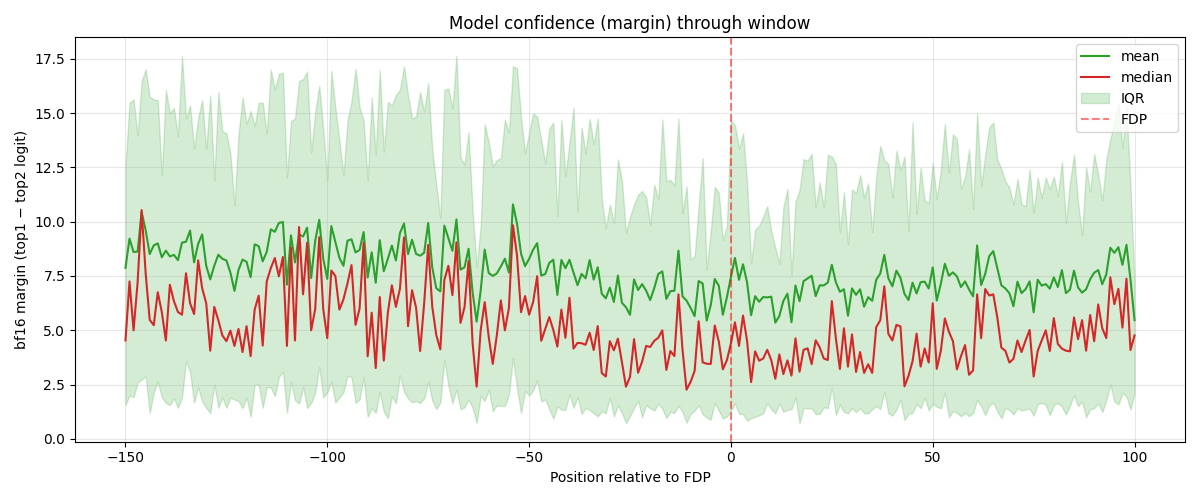
\includegraphics[width=0.85\textwidth]{figures/fig_margin.png}
\caption{Медиана top-1/top-2 margin-а (нат) bf16-модели как функция
позиции относительно FDP.}
\label{fig:margin}
\end{figure}

\begin{table}[H]
\centering
\caption{Медиана margin-а по позициям относительно FDP.}
\label{tab:margin}
\begin{tabular}{lcccccc}
\toprule
Позиция rel. FDP & $-50$ & \textbf{$-10$} & $-1$ & 0 & $+1$ & $+10$ \\
\midrule
Median margin (нат) & 5,72 & \textbf{2,62} (min) & 3,62 & 4,39 & 5,37 & 3,62 \\
\bottomrule
\end{tabular}
\end{table}

Минимум margin-а --- в окрестности FDP$-10$. Гипотеза подтверждается:
flip случается там, где \textbf{модель сама себе не уверена}, а не
там, где квант-шум необычно большой. Как только контекст подводит
модель к сложному шагу с маленьким margin-ом, даже накопленной ошибки
хватает для flip-а. После первого flip-а контексты bf16 и fp8 уже
разные, и расхождение становится compound.

\subsection*{4.8 Что меняется с ростом размера модели}

Если outlier-каналы --- свойство весов, что будет на большей модели?
Сравниваем Qwen3-1.7B и Qwen3-4B:

\begin{figure}[H]
\centering
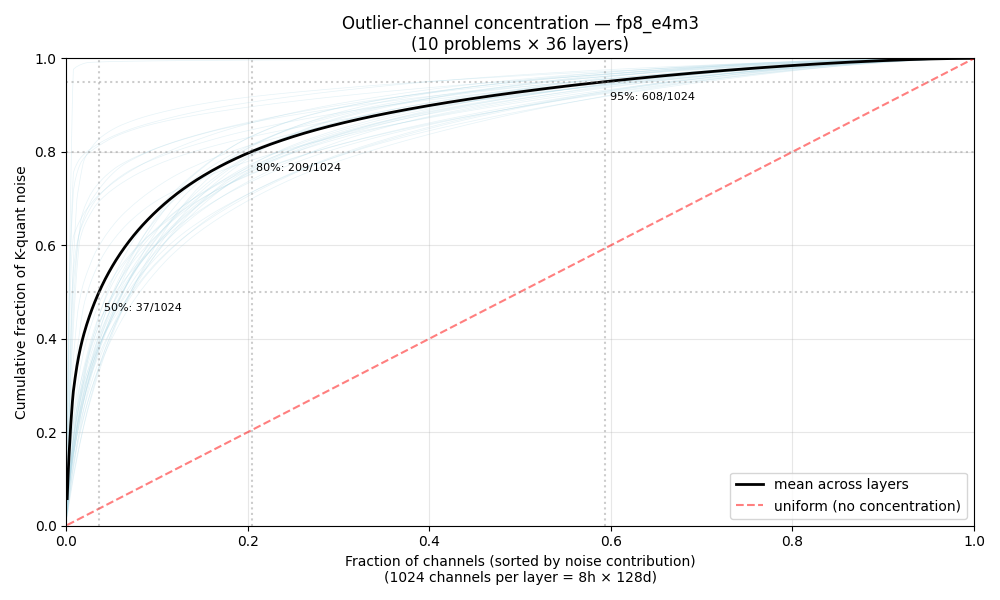
\includegraphics[width=0.82\textwidth]{figures/fig_qwen4b.png}
\caption{Концентрация для Qwen3-4B (10 задач, fp8\_e4m3): top-10
покрывают 21\% против 51,7\% на Qwen3-1.7B.}
\label{fig:qwen4b}
\end{figure}

\begin{table}[H]
\centering
\caption{Кросс-масштабное сравнение.}
\label{tab:scale}
\begin{tabular}{lcc}
\toprule
Metric & Qwen3-1.7B & Qwen3-4B \\
\midrule
top-1 channel & 10,3~\% & \textbf{3,6~\%} ($\div 3$) \\
top-10 fraction & 51,7~\% & \textbf{21,0~\%} ($\div 2{,}5$) \\
\# ch для 50\% & 8 & 56 ($\times 7$) \\
\bottomrule
\end{tabular}
\end{table}

С ростом hidden state шум распределяется по бóльшему числу каналов ---
концентрация падает. Уже здесь становится подозрительно, что
«красивая» цифра 51,7\% \textit{специфична для 1.7B}, а не universal.

\paragraph{Итог части 4 и переход к части 5.} Mechanism проложен:
неравномерный шум $K$ $\to$ нелинейно усиленный сдвиг attention $\to$
каскад через слои $\to$ flip в точке минимального margin-а. Сразу
напрашивается гипотеза: если 10 каналов несут половину шума, давайте
\textbf{защитим эти 10 каналов в bf16} --- остальное оставим в FP8.
Этот рецепт и проверяем в части~5.

\clearpage

% =====================================================================
% ЧАСТЬ 5 — ЗАЩИТА
% =====================================================================
\section*{Часть~5. Защитный рецепт: естественная гипотеза, которая не сработала}
\addcontentsline{toc}{section}{Часть~5. Защитный рецепт}

\paragraph{Цель главы.} Проверить гипотезу из конца части~4
(«защитим top-10 каналов в bf16»). Сначала в лаборатории (TF-режим),
потом в реальной production-ситуации (AR-генерация). Заранее скажем
результат: \textit{лабораторно работает, в production --- нет}.

\subsection*{5.1 Формулировка рецепта}

Для каждого слоя выбираем $N$ каналов с наибольшим
$\max_t |K_\text{pre}[t, h, c]|$ и сохраняем их в bf16. Остальные
$1024 - N$ каналов квантизуются как обычно. Цена защиты ---
$N/1024$ дополнительной bf16-памяти.

\subsection*{5.2 Лабораторная проверка: рецепт работает (Qwen3-1.7B, TF)}

Все цифры в этом разделе получены на Qwen3-1.7B, 80 задачах, в
teacher-forced режиме (одиночный forward через captured window).

\begin{figure}[H]
\centering
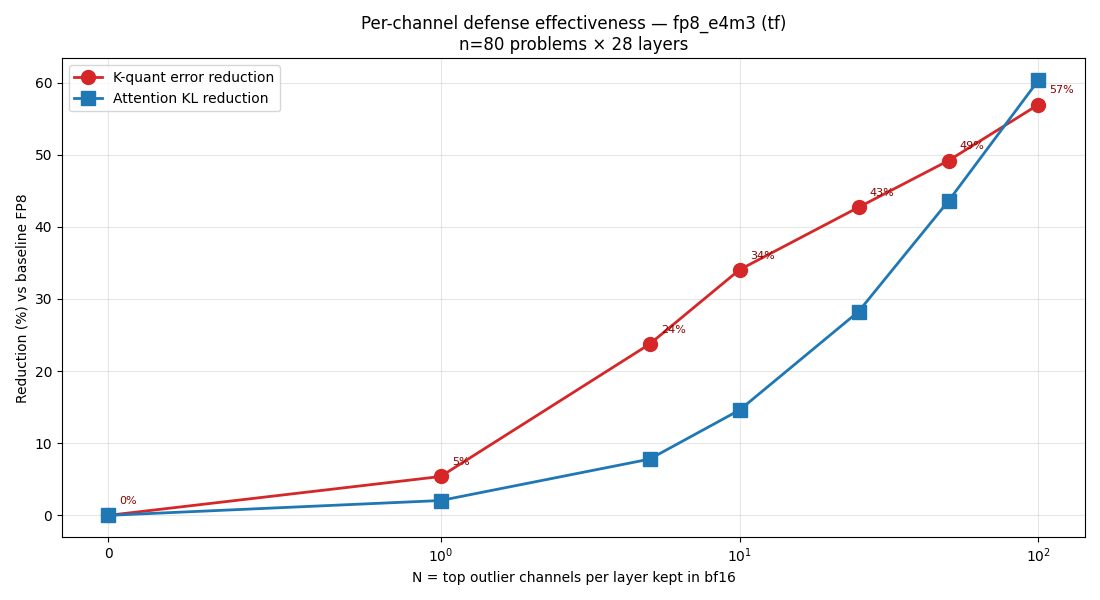
\includegraphics[width=0.82\textwidth]{figures/fig_defense_lab.png}
\caption{Лабораторная эффективность per-channel защиты fp8\_e4m3:
восстановление K-ошибки и attention-KL как функция числа защищённых
каналов $N$.}
\label{fig:deflab}
\end{figure}

\begin{table}[H]
\centering
\caption{Лабораторная эффективность защиты для fp8\_e4m3.}
\label{tab:defense}
\begin{tabular}{cccc}
\toprule
$N$ & \% каналов & $\Delta$ K-error & $\Delta$ attention-KL \\
\midrule
1   & 0,10~\% & $-5{,}4$~\% & $-2{,}1$~\% \\
5   & 0,49~\% & $-23{,}7$~\% & $-7{,}8$~\% \\
\textbf{10} & \textbf{0,98~\%} & \textbf{$-34{,}1$~\%} & \textbf{$-14{,}6$~\%} \\
25  & 2,44~\% & $-42{,}7$~\% & $-28{,}3$~\% \\
100 & 9,77~\% & $-57{,}0$~\% & $-60{,}3$~\% \\
\bottomrule
\end{tabular}
\end{table}

При $N = 10$ (\,$\approx 1\%$ каналов в bf16) восстанавливается 34\%
K-ошибки и 15\% attention-shift KL. Это очень сильный TF-метрический
результат, который и подкупает.

\subsection*{5.3 Рецепт работает только на простых линейных квантизациях}

Тот же $N = 10$ на разных форматах:

\begin{table}[H]
\centering
\caption{Эффект защиты $N=10$ по форматам.}
\label{tab:hqqdef}
\begin{tabular}{lcccc}
\toprule
$N=10$ & fp8\_e4m3 & fp8\_e5m2 & hqq\_int4 & hqq\_int2 \\
\midrule
$\Delta$ K-error & $\mathbf{-34{,}1\%}$ & $\mathbf{-33{,}1\%}$ & $\mathbf{+5{,}7\%}$ & $\mathbf{+6{,}7\%}$ \\
\bottomrule
\end{tabular}
\end{table}

Видим: на FP8 защита помогает ($\sim -34\%$ на e4m3 и e5m2). На HQQ
\textit{ухудшает} ($+5{,}7\%$ для INT4, $+6{,}7\%$ для INT2). Причина:
у HQQ уже встроен per-group scale + zero-point, который сам адаптируется
к outlier-ам внутри группы. Принудительная защита bf16-каналом ломает
эту адаптивную калибровку и добавляет шума, а не убирает.

\textbf{Вывод.} Per-channel изоляция работает только на простых линейных
схемах (min-max / abs-max на тензор --- как в per-tensor FP8). На
форматах с outlier-aware-калибровкой (HQQ) рецепт неприменим.

\subsection*{5.4 Production-проверка: рецепт провалился в AR-генерации}

Теперь самое важное. Лабораторная метрика (TF) --- это single forward
через captured window. Production-инференс --- это \textit{authorregressive}
генерация: на каждом шаге модель видит \textit{один} новый K-токен и
обновляет кэш. Будет ли работать та же защита здесь?

На 10 свежих MATH-500 задачах запустили реальную AR-генерацию (max
100 токенов, greedy):

\begin{figure}[H]
\centering
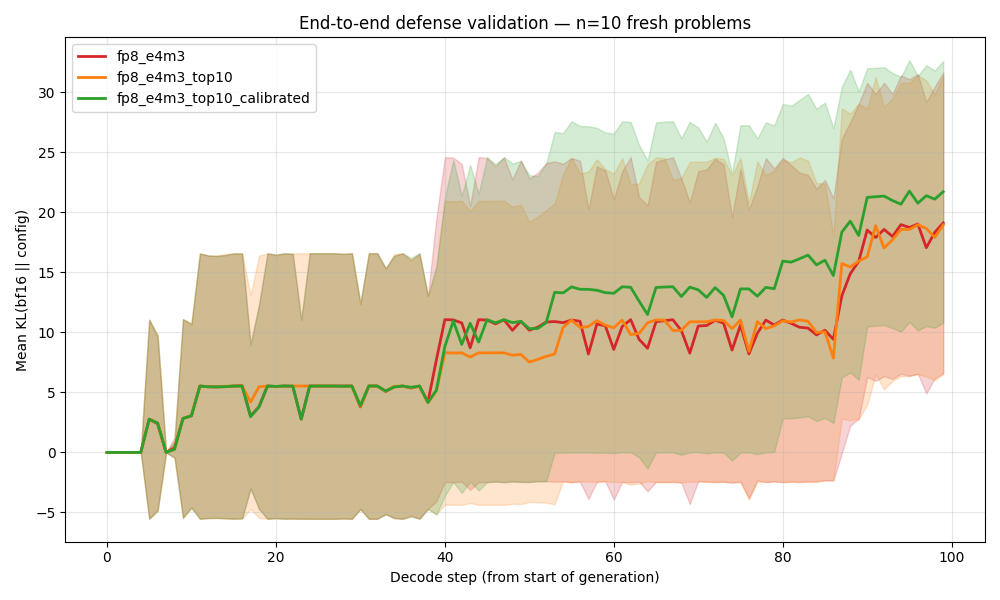
\includegraphics[width=0.85\textwidth]{figures/fig_defense_ar.png}
\caption{Mean logit-KL между bf16 и fp8 траекториями как функция шага
декодирования.}
\label{fig:defar}
\end{figure}

\begin{table}[H]
\centering
\caption{End-to-end AR-валидация защиты (10 задач, 100 токенов).}
\label{tab:arval}
\small
\begin{tabular}{lccc}
\toprule
Метрика & fp8 baseline & top-10 per-step & top-10 calibrated \\
\midrule
Mean first divergence step & 57,5  & 58,9 ($+1{,}4$) & 52,4 ($-5{,}1$) \\
Token agreement @ 100      & 0,658 & 0,668 ($+0{,}010$) & 0,600 ($-0{,}058$) \\
Mean logit KL              & 8,749 & 8,539 ($-2{,}4$~\%) & 10,329 ($+18$~\%) \\
\bottomrule
\end{tabular}
\end{table}

\textbf{Результат:} лабораторные $-15\%$ attn-KL превращаются в
$-2{,}4\%$ logit-KL --- это внутри уровня шума. Token agreement растёт
лишь на 1~п.п. (тоже шум). Calibrated SmoothQuant-style вариант (где
outlier-каналы зафиксированы на prefill и не пересчитываются) делает
\textit{хуже}: $+18\%$ logit-KL.

\paragraph{Почему рецепт провалился.} На decode-шаге attention видит
\textit{только один} новый K-токен; identity outlier-каналов на одном
векторе нестабильна между шагами. K-error recovery в одной позиции не
пропагирует через compound softmax $\to$ cascade $\to$ logits в AR.
Argmax flip начинается уже с $\sim$40-го декод-шага, несмотря на
формально работающую защиту.

\paragraph{Итог части 5 (первый фундаментальный результат, Ф.2).}
Защитный рецепт привлекательно выглядит в TF-метрике, но в реальной
AR-генерации не работает. Это и есть наш \textbf{структурный закон
``lab $\to$ production''-разрыва}: одиночный forward систематически
переоценивает практическую пользу любого quant-defense рецепта, потому
что compound AR разрушает single-position recovery. Дальше возникает
естественный вопрос: насколько вообще численные результаты, полученные
на одной модели (Qwen3-1.7B), отражают свойство transformer attention в
целом? Это проверяется в части~6.

\clearpage

% =====================================================================
% ЧАСТЬ 6 — КРОСС-СЕМЕЙНАЯ
% =====================================================================
\section*{Часть~6. Кросс-семейная валидация и количественный закон recovery $\approx 0{,}65 \cdot$ concentration}
\addcontentsline{toc}{section}{Часть~6. Кросс-семейная валидация}

\paragraph{Цель главы.} Прогнать тот же pipeline на 4 моделях из разных
семейств и выяснить две вещи: (1) какие из количественных результатов
части~4 универсальны для transformers, а какие --- свойство одной
модели, и (2) есть ли количественный закон, связывающий концентрацию
шума с эффективностью защиты, который выполняется межсемейно. Эта глава
содержит третий фундаментальный результат работы (Ф.3).

\subsection*{6.1 Какие модели взяли}

\begin{table}[H]
\centering
\caption{Тестируемые модели.}
\label{tab:models}
\begin{tabular}{llcc}
\toprule
Модель & Семейство & Layers & KV-heads \\
\midrule
Qwen3-1.7B & Qwen3 (главная модель работы) & 28 & 8 \\
Qwen2.5-1.5B-Instruct & Qwen2 & 28 & 2 (GQA-2) \\
DeepSeek-R1-Distill-Qwen-1.5B & Qwen2 base + R1 distillation & 28 & 2 \\
SmolLM2-1.7B-Instruct & \textbf{Llama-3-derived} (не Qwen) & 24 & 8 \\
Qwen3-4B & Qwen3 (бóльший) & 36 & 8 \\
\bottomrule
\end{tabular}
\end{table}

Идея: Qwen3-1.7B --- baseline; Qwen2.5 и DeepSeek-R1-Distill --- та же
семейная ветка, проверка повторяемости; SmolLM2 --- принципиально
другое семейство (Llama-3), главный «контрольный» тест.

\subsection*{6.2 Что НЕ зависит от модели: magnitude K-ошибки}

\begin{figure}[H]
\centering
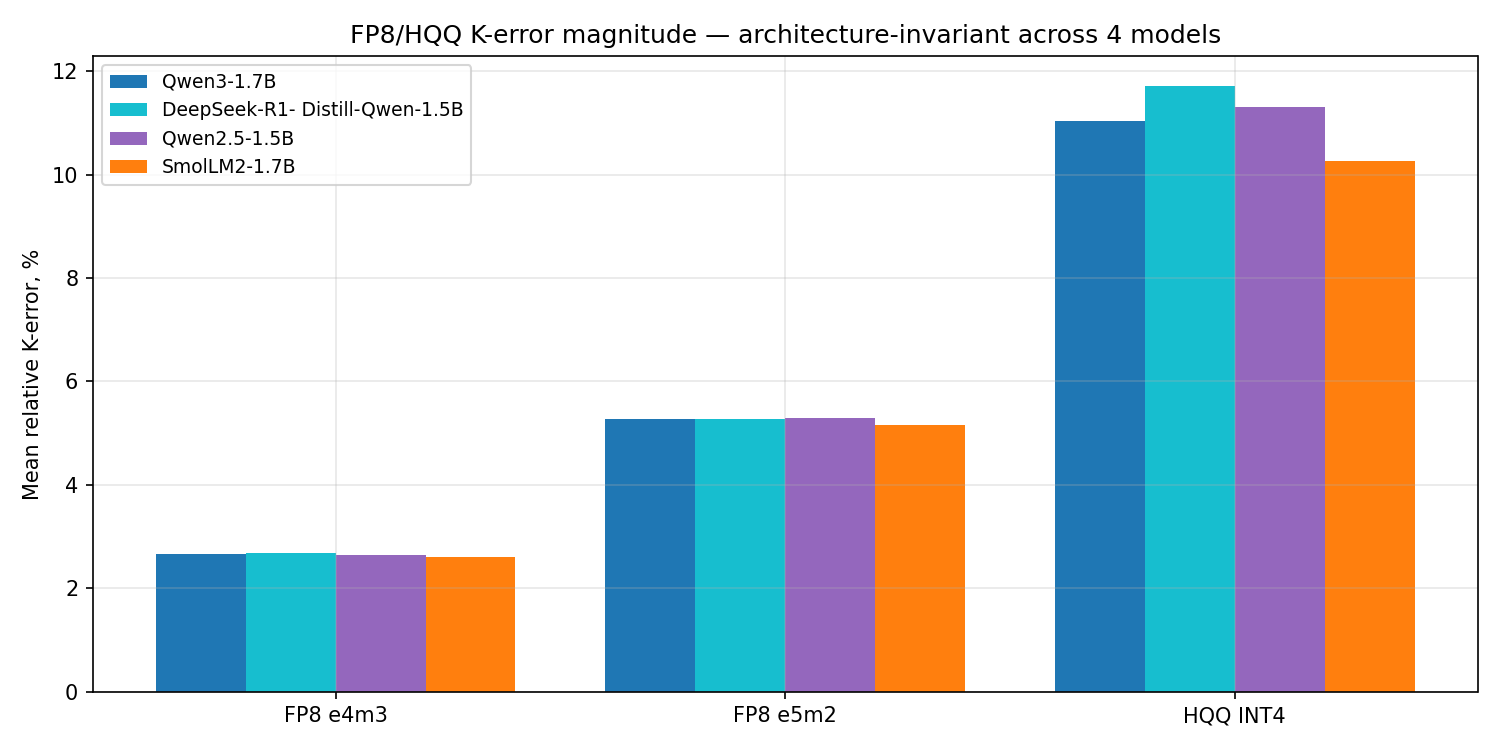
\includegraphics[width=0.95\textwidth]{figures/fig_kerr_invariance.png}
\caption{Mean relative K-error по 4 моделям для трёх форматов
квантизации. Magnitude совпадает с точностью $\sim 3\%$.}
\label{fig:kerrinv}
\end{figure}

\textbf{Magnitude} K-ошибки ($\sim 2{,}65\%$ для fp8\_e4m3, $\sim 5{,}25\%$
для fp8\_e5m2, $\sim 10\%$ для HQQ INT4) тождественен на всех 4 моделях.
Это структурное свойство FP8 round-to-nearest, оно не зависит от
модели. Этот результат как ожидался.

\subsection*{6.3 Что СИЛЬНО зависит от модели: концентрация шума}

\begin{figure}[H]
\centering
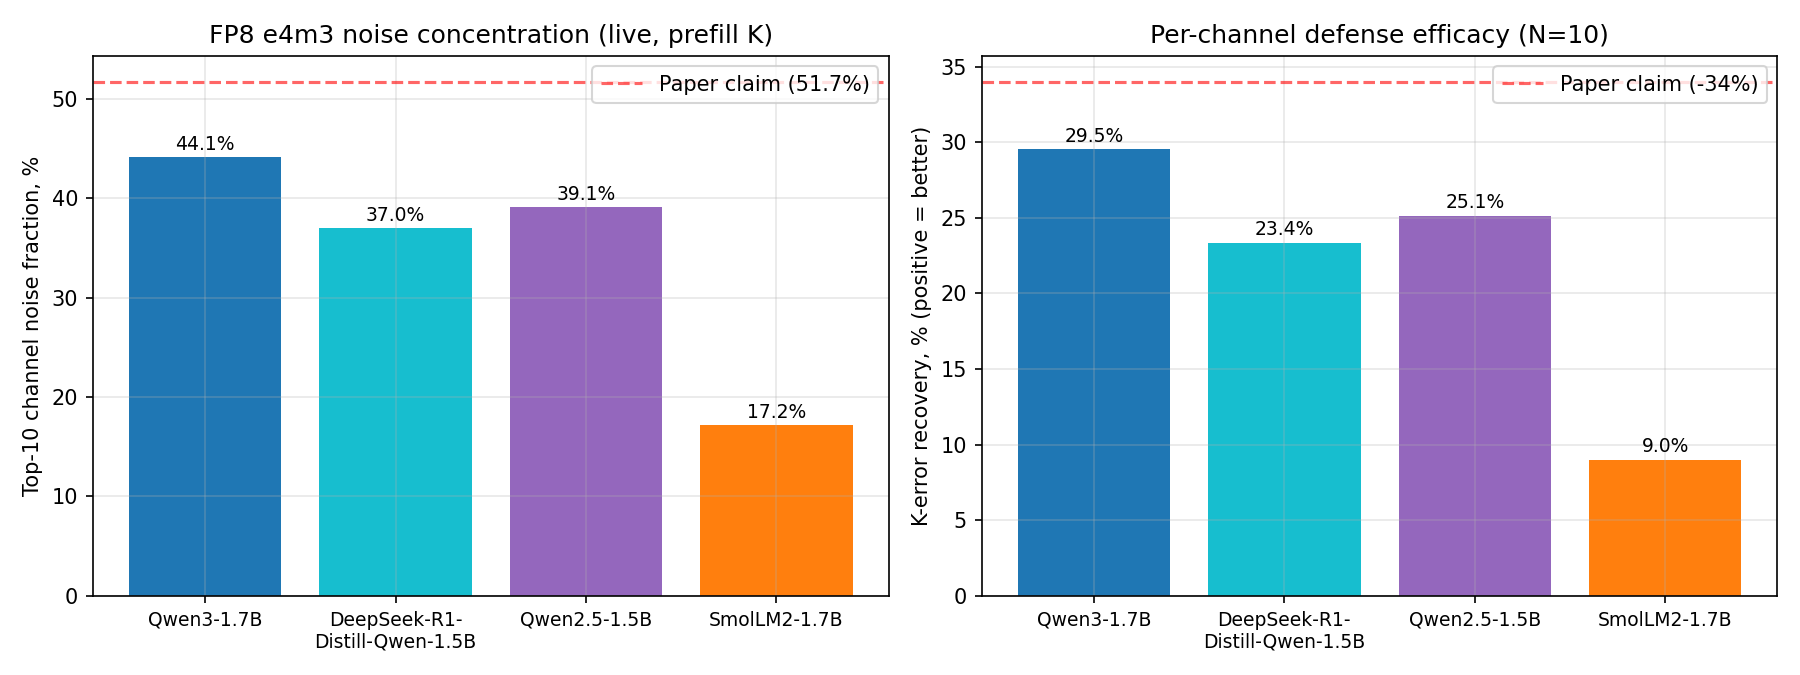
\includegraphics[width=\textwidth]{figures/fig_cross_model.png}
\caption{Cross-model сравнение fp8\_e4m3. Слева: концентрация top-10
каналов; красная линия --- значение на Qwen3-1.7B (51,7\%) для
сравнения. Справа: эффективность защиты $N = 10$; красная линия ---
значение на Qwen3-1.7B ($-34\%$).}
\label{fig:crossmodel}
\end{figure}

\begin{figure}[H]
\centering
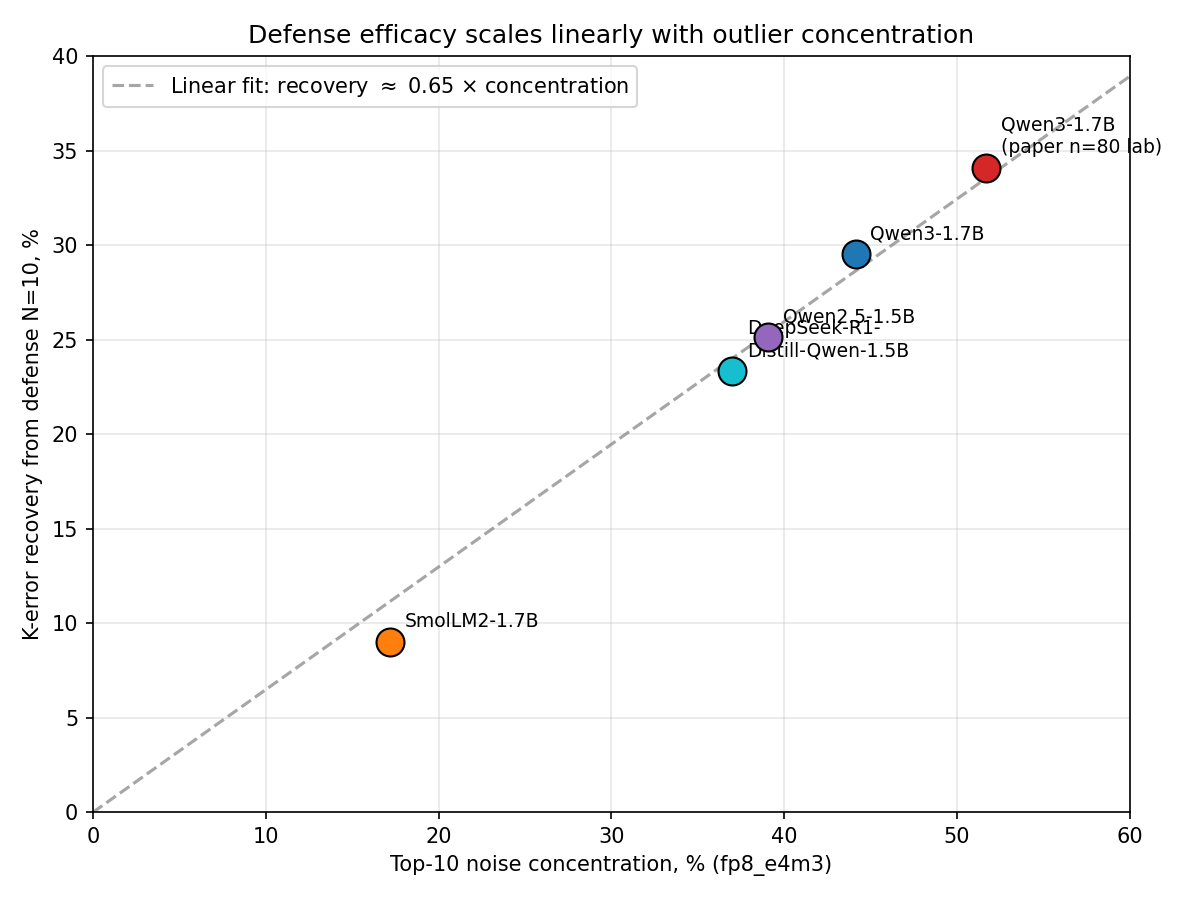
\includegraphics[width=0.82\textwidth]{figures/fig_recovery_vs_concentration.png}
\caption{Линейная зависимость восстановления K-ошибки от концентрации:
\texttt{recovery $\approx$ 0,65 $\times$ concentration}.}
\label{fig:recvsconc}
\end{figure}

\begin{table}[H]
\centering
\caption{Cross-model результаты на свежих задачах.}
\label{tab:cross}
\small
\begin{tabular}{lccc}
\toprule
Модель & top-1 & top-10 & defense $N=10$ \\
\midrule
Qwen3-1.7B ($n=20$) & 9,8~\% & \textbf{44,1~\%} & \textbf{$-29{,}5~\%$} \\
DeepSeek-R1-Distill-Qwen-1.5B ($n=10$) & 7,5~\% & 37,0~\% & $-23{,}4~\%$ \\
Qwen2.5-1.5B ($n=5$) & 12,8~\% & 39,1~\% & $-25{,}1~\%$ \\
\textbf{SmolLM2-1.7B} (Llama-arch, $n=5$) & 2,9~\% & \textbf{17,2~\%} & \textbf{$-9{,}0~\%$} \\
\bottomrule
\end{tabular}
\end{table}

\textbf{Простыми словами.} У Qwen-семейства 10 каналов из 1024 несут
37--44\% шума, и защита этих каналов даёт $-23\ldots -29\%$ K-error.
На SmolLM2 (Llama-arch) \textit{те же} 10 каналов несут только 17\%
шума, и защита даёт всего $-9\%$ --- почти ничего. Recovery
масштабируется линейно: \texttt{recovery $\approx$ 0,65 $\times$
top10\_fraction}.

\subsection*{6.4 Фундаментальный результат Ф.3: количественный закон concentration $\to$ recovery}

Когда мы строим зависимость восстановления K-ошибки от концентрации
шума по 4 моделям (рис.~\ref{fig:recvsconc}), точки выстраиваются вдоль
прямой:
\[
\text{recovery} \;\approx\; 0{,}65 \cdot \text{top10\_fraction}.
\]

Это \textbf{количественный межсемейный закон}, найденный в данной
работе. Он связывает структурную характеристику модели (концентрация
шума в top-10 каналах) с эффективностью защитного приёма (восстановление
K-ошибки) с одним и тем же коэффициентом на четырёх архитектурно разных
моделях. Это не подгонка под одну модель и не корреляция «вообще» ---
это конкретное численное правило с предсказательной силой:

\begin{itemize}[leftmargin=*]
\item Если на новой модели измерить top-10 fraction за один
  calibration-прогон, можно \textbf{априорно предсказать пользу}
  per-channel защиты до её внедрения.
\item Если top-10 fraction $< 25\%$ --- ожидаемое восстановление ниже
  16\%, метод бесполезен (как на SmolLM2: 17\% $\to$ -9\%).
\item Если top-10 fraction $\sim 50\%$ --- ожидаемое восстановление
  около -32\% (как на Qwen3-1.7B: 51,7\% $\to$ -34\%).
\end{itemize}

\paragraph{Сопутствующий негативный результат.} Цифра «top-10 = 51,7\%»,
полученная в части~4 на Qwen3-1.7B, на других моделях не воспроизводится
в той же величине (17--44\%). Концентрация --- семейно-зависимая
характеристика; универсально только \textit{качественное} утверждение
«концентрация существенно выше равномерной» (\(\gg 10/1024 = 0{,}98\%\)),
а количественно --- зависит от модели. Это нужно учитывать при любых
обобщениях типа «такая-то доля шума концентрируется в transformer
attention».

\begin{quote}
\textbf{Слабая предпосылка для дальнейшего изучения.} Возможно, на
отдельных внутренних слоях не-Qwen моделей можно найти
полу-концентрированные подсистемы, защита которых имела бы смысл. Эта
гипотеза за рамками данной работы.
\end{quote}

\subsection*{6.5 Сводка: что работает на практике, а не в теории}

\textbf{Универсально (подтверждено на всех 4 моделях):}
\begin{itemize}[leftmargin=*]
\item Magnitude K-ошибки определяется только форматом квантизации,
  а не моделью ($\sim 2{,}65\%$ для fp8\_e4m3 на всех 4 моделях).
\item HQQ распределяет шум в 4--5 раз более равномерно, чем FP8 ---
  отношение top-10 fraction FP8/HQQ устойчиво $\in [3{,}9,\, 4{,}9]$ на
  всех 4 моделях.
\item Количественный закон \(\text{recovery} \approx 0{,}65 \cdot
  \text{top10\_fraction}\) --- линейная зависимость с одним
  коэффициентом на всех 4 моделях.
\item Воспроизводимость outlier-каналов между сидами (Jaccard 0,879).
\item Mechanism-цепочка из части~4 (softmax-усиление в $\sim 100$ раз,
  margin-минимум вблизи FDP, насыщение KL по $\tau \sim 130$) ---
  качественно сохраняется межсемейно.
\end{itemize}

\textbf{Зависит от модели / Qwen3-1.7B specific:}
\begin{itemize}[leftmargin=*]
\item Численное значение top-10 fraction (17--52\% между моделями).
\item Численная величина recovery от защиты (-9\% до -34\%).
\item Конкретный ranking слоёв (L3, L4 как victim layers на Qwen3-1.7B
  не обязан совпадать с другими моделями).
\item Конкретные численные значения $\tau$, $K_\infty$.
\end{itemize}

\textbf{Не работает на любой проверенной модели:}
\begin{itemize}[leftmargin=*]
\item Per-channel defense в реальной AR-генерации
  (Ф.2 из части~5: -2,4\% logit-KL на Qwen3-1.7B,
  argmax-flip с $\sim 40$-го шага).
\item Per-channel defense на HQQ (ломает per-group калибровку).
\item Прогноз FDP по prompt-only признакам ($R^2 < 0$ на двух разных
  моделях --- см. часть~7).
\end{itemize}

\paragraph{Итог части 6 и переход к части 7.} Mechanism-картина из
части~4 универсальна качественно, но численно --- семейно-зависима.
Найденный количественный закон concentration~$\to$~recovery даёт
инженерам априорный критерий применимости защиты. Возникает следующий
практический вопрос: \textit{можно ли заранее предсказать, на какой
задаче модель сломается под FP8?} Если да --- можно просто
перенаправить «хрупкие» задачи на bf16, минуя проблему AR-разрыва. Это
и есть задача части~7.

\clearpage

% =====================================================================
% ЧАСТЬ 7 — FDP PREDICTOR
% =====================================================================
\section*{Часть~7. ML-прогноз точки первого расхождения (FDP)}
\addcontentsline{toc}{section}{Часть~7. ML-прогноз FDP}

\paragraph{Цель главы.} Построить ML-модель, которая по K-матрицам
предсказывает позицию FDP (или хотя бы её бакет). Параллельно эта задача
служит \textit{косвенным валидатором} mechanism-claim-ов из части~4:
если FDP действительно определяется тем, что мы описали, то ML должно
суметь её предсказать.

\subsection*{7.1 Задача и dataset}

\textbf{Target:} \texttt{fdp\_token\_idx} --- целое число в диапазоне
$\sim 0$--1200 для каждой задачи (problem, fp8\_e4m3) на Qwen3-1.7B.
\textbf{Input:} K-матрицы из decode-window (или их статистики).
\textbf{Dataset:} 80 задач AIME-24/MATH-500, 5-fold cross-validation.

\subsection*{7.2 Шесть базовых экспериментов}

\begin{table}[H]
\centering
\caption{Сводка по 6 подходам.}
\label{tab:6exp}
\small
\begin{tabular}{clccc}
\toprule
\# & Подход & $R^2$ & MAE (tokens) & Spearman \\
\midrule
0 & Mean baseline & $\approx 0$ & 309 & --- \\
1 & GBM на decode-window features (980-d) & 0,860 $\pm$ 0,02 & 102 & 0,852 \\
2 & MLP на тех же features & 0,813 $\pm$ 0,07 & 113 & 0,839 \\
A & GBM на \textit{prompt-only} prefill K & $\mathbf{-0{,}348}$ & 381 & $-0{,}066$ \\
B & Two-stage (clf + 2 регрессии) & 0,818 & 106 & 0,830 \\
\textbf{D} & \textbf{1D-CNN на raw K-матрицах} & \textbf{0,976 $\pm$ 0,02} & \textbf{43} & 0,888 \\
E1 & Cross-quant $\to$ fp8\_e5m2 & 0,955 & 50 & 0,907 \\
E2 & Cross-quant $\to$ hqq\_int4 & 0,851 & 123 & 0,864 \\
F & Cross-model Qwen3 $\to$ DeepSeek (prefill) & $\mathbf{-4{,}002}$ & 382 & 0,333 \\
\bottomrule
\end{tabular}
\end{table}

\begin{figure}[H]
\centering
\includegraphics[width=0.95\textwidth]{../../outputs/kv_capture/qwen3-1.7b/analysis/plots/fdp_predictor_comparison.png}
\caption{Сравнение 6 подходов на одной шкале $R^2$.}
\label{fig:6cmp}
\end{figure}

\textbf{Два неочевидных результата.}

\textit{Эксперимент A провалился ($R^2 < 0$).} GBM на признаках,
извлечённых только из prefill K (то есть из промпта до начала
генерации), даёт \textit{отрицательное} $R^2$. То же самое в
эксперименте F при cross-model self-CV. Вывод: \textbf{промпт сам по
себе не предсказывает FDP}. FDP --- compound emergent property,
проявляется только во время декодирования. Это согласуется с
mechanism-картинкой из части~4 (накопление через каскад).

\textit{Эксперимент D даёт R² = 0,98.} 1D-CNN, обученный
непосредственно на raw K-матрицах из decode-window, даёт R² = 0,98 ---
это требует отдельной проверки на честность (см. 7.4).

\subsection*{7.3 Какие признаки реально несут signal (Qwen3-1.7B only)}

\begin{quote}
\textbf{Важно.} Все измерения важности признаков ниже сделаны
исключительно на Qwen3-1.7B fp8\_e4m3 (80 задач). На других моделях
ranking может отличаться --- это не проверялось.
\end{quote}

\begin{figure}[H]
\centering
\includegraphics[width=\textwidth]{../../outputs/kv_capture/qwen3-1.7b/analysis/plots/fdp_predictor_scatter.png}
\caption{Scatter predicted vs true FDP для GBM и MLP (5-fold CV).}
\label{fig:fdpscatter}
\end{figure}

\begin{table}[H]
\centering
\caption{Распределение важности по типам признаков (Qwen3-1.7B GBM).}
\label{tab:featimp}
\begin{tabular}{lc}
\toprule
Тип признака & Важность \\
\midrule
\texttt{mean\_abs} per (L, h) & 35,8~\% \\
\texttt{std} per (L, h) & 32,9~\% \\
\texttt{max\_abs} per (L, h) & 23,3~\% \\
\texttt{top1\_ch\_lh} & 7,3~\% \\
\texttt{top10\_frac} per L & 0,6~\% \\
\texttt{top1\_frac} per L & 0,04~\% \\
\bottomrule
\end{tabular}
\end{table}

\textbf{Top-5 предсказательных слоёв:} L4 (22,3\%), L3 (20,7\%), L25,
L18, L7. Те же слои L3 и L4 ранее выделились в части~4.5 как наиболее
«хрупкие» по logit-impact при single-layer ablation --- то есть
независимое ML-измерение \textit{подтверждает} наш mechanism-вывод о
центральности этих слоёв для Qwen3-1.7B.

\textbf{Неожиданное наблюдение:} amplitude-метрики
(\texttt{mean\_abs}, \texttt{std}, \texttt{max\_abs}) дают 92\% важности,
а concentration-метрики --- меньше 1\%. То есть для ML-предсказания
FDP важнее «насколько большие значения сейчас в $K$», а не «как они
сконцентрированы». Для Qwen3-1.7B amplitude $>$ concentration; обобщать
пока нельзя.

\subsection*{7.4 Проверка на overfitting (4 теста)}

R² = 0,98 на $n=80$ --- подозрительно. Делаем 4 независимых проверки.

\begin{figure}[H]
\centering
\includegraphics[width=\textwidth]{../../outputs/kv_capture/qwen3-1.7b/analysis/plots/fdp_overfitting_check.png}
\caption{Слева: learning curve train vs val $R^2$. Справа: train vs val
$R^2$ по эпохам.}
\label{fig:overfit}
\end{figure}

\begin{table}[H]
\centering
\caption{Четыре теста на overfitting.}
\label{tab:overfit}
\small
\begin{tabular}{lccl}
\toprule
Тест & Real $R^2$ & Контроль & Вердикт \\
\midrule
1. Label shuffle & 0,971 & $\mathbf{-0{,}305}$ & gap $+1{,}28$ = signal \\
4. Random input & 0,97 & $\mathbf{-0{,}123}$ & не fitting noise \\
2. Learning curve gap при $n=64$ & train 0,99, val 0,98 & \textbf{0,011} & здоровое generalization \\
3. Epoch curves & val $0{,}94 \to 0{,}99$ monotone & no divergence & overfit pattern отсутствует \\
\bottomrule
\end{tabular}
\end{table}

Если перемешать labels, R² падает до $-0{,}3$. Если подать на вход
случайный гауссов шум, R² $\to -0{,}12$. Train-val gap уменьшается с
ростом $n$ (с 0,31 при $n=20$ до 0,011 при $n=64$) --- это
противоположность overfitting-у. \textbf{CNN R² = 0,97--0,98 ---
реальный signal}, не запоминание.

\subsection*{7.5 Тест на 5 MATH-500 задачах: distribution shift и переформулировка}

In-distribution CV дала R² = 0,98. Что будет на
задачах MATH-500 (idx 80--84), которых вообще не было в обучении?

\begin{figure}[H]
\centering
\includegraphics[width=0.82\textwidth]{../../outputs/kv_capture/qwen3-1.7b/analysis/plots/cnn_new_problems_test.png}
\caption{CNN-предсказание FDP на 5 свежих MATH-500 задачах.}
\label{fig:cnnfresh}
\end{figure}

\begin{table}[H]
\centering
\caption{Per-problem результат на 5 свежих задачах.}
\label{tab:fresh5}
\begin{tabular}{ccccl}
\toprule
Problem & True FDP & Predicted & Error & Вердикт \\
\midrule
80 & 63 & 63 & \textbf{0} & $\checkmark$ \\
81 & 8 & 32 & $+24$ & близко \\
\textbf{82} & 99 & \textbf{285} & $\mathbf{+186}$ & выброс \\
83 & 37 & 44 & $+7$ & $\checkmark$ \\
84 & 45 & 29 & $-16$ & $\checkmark$ \\
\bottomrule
\end{tabular}
\end{table}

\textbf{Метрики:} MAE~$=$~47 (12 без выброса \#82); $R^2 = -6{,}88$;
Spearman~$\rho = 0{,}70$.

R² катастрофически плохой из-за distribution shift: в train medianа
FDP = 585, а в test все задачи $< 100$. Модель видела в обучении в
основном «долгие» FDP и считает короткие выбросами. 4 из 5 предсказаний
точные (MAE $\le 24$), один выброс (\#82) разрушает R², но \textbf{не
ranking}: $\rho = 0{,}70$.

\paragraph{Переформулировка: ranking вместо regression.} Для
production-применения не нужно предсказывать точную позицию FDP в
токенах --- достаточно \textit{упорядочить} задачи по тому, какие
сломаются раньше. Это ranking-task, и наш предсказатель её решает.
Метрика --- Spearman $\rho$ или NDCG@$K$. Под эту метрику CNN
работоспособен и на свежих задачах.

\textbf{Применение:}
\begin{enumerate}[label=\arabic*.,leftmargin=*]
\item \textbf{Online canary} в inference-loop: каждые 20--40 декод-шагов
  прогоняем $K$ через CNN, получаем «оценку доверия до FDP». При
  предсказании $< 30$ шагов --- переключаем запрос на bf16-cache.
\item \textbf{Adaptive batching:} после prefill ранжируем batch по
  предсказанной хрупкости (близости FDP), top-$K$ самых хрупких задач
  выносим в отдельный bf16-batch, остальные оставляем в FP8.
\item \textbf{Quality SLA gating:} отказывать в FP8-инференсе задачам,
  попадающим в top-5\% самых хрупких (лучше отказ, чем сломанный
  ответ).
\end{enumerate}

\subsection*{7.6 Cross-model: предсказатель не переносится напрямую}

\begin{table}[H]
\centering
\caption{Метрики предсказателя, обученного и тестированного на
DeepSeek-R1-Distill.}
\label{tab:deepseekpred}
\begin{tabular}{lccc}
\toprule
Predictor on DeepSeek & $R^2$ & MAE & Spearman \\
\midrule
GBM & $-3{,}90$ & 22 & \textbf{0,94} \\
MLP & 0,17 & 20 & 0,57 \\
CNN & $-0{,}39$ & 29 & 0,41 \\
\bottomrule
\end{tabular}
\end{table}

$R^2$ снова катастрофический, потому что распределение FDP на DeepSeek
сильно скошено (median FDP $=$ 7 vs Qwen3 median $=$ 585). Spearman
GBM = 0,94 --- ranking работает.

\begin{quote}
\textbf{Чего нельзя заявить.} Тот факт, что у DeepSeek-R1-Distill median
FDP = 7 при FP8, а у Qwen3-1.7B = 585, \textit{не означает}, что
reasoning-distillation универсально делает модель более уязвимой к
квантизации. FDP --- это позиция расхождения той же модели с её
собственным bf16-baseline. Разные модели могут просто по-разному
стартовать генерацию, иметь разные распределения длины выхода, разные
margin-ы. Корректное сравнение хрупкости между моделями требует
контроля как минимум на длину выхода, формат промпта, базовую энтропию
первых токенов --- мы этого не делали.

Корректная интерпретация: на нашем наборе из 80 задач MATH-500
DeepSeek-R1-Distill чаще, чем Qwen3-1.7B, теряет совпадение со своим
bf16-baseline в первых десятках токенов под FP8 e4m3. Это факт о двух
конкретных моделях на одном датасете, а не «общее свойство
reasoning-distillation».
\end{quote}

\textbf{Прямой transfer весов CNN} (обучили на Qwen3, проверили на
DeepSeek prefill features): $R^2 = -4{,}0$. Архитектуры различаются
числом KV-heads (8 vs 2) и формой K-распределения --- feature-space
разный, прямой transfer без re-training не работает.

\subsection*{7.7 Bucket-classifier на свежих задачах}

Чтобы обойти проблему distribution shift, переформулируем задачу как
4-классовую классификацию: бакеты по квартилям training FDP-распределения
($\le 533$, $(533, 585]$, $(585, 1021]$, $> 1021$).

\begin{figure}[H]
\centering
\includegraphics[width=\textwidth]{../../outputs/kv_capture/qwen3-1.7b/analysis/plots/cnn_buckets_test.png}
\caption{Bucket-классификатор на 6 задачах math-500: confusion (слева),
predicted probabilities (справа).}
\label{fig:bucket}
\end{figure}

\begin{table}[H]
\centering
\caption{Per-problem результат bucket-классификатора (idx 81--86).}
\label{tab:bucket}
\begin{tabular}{ccccc}
\toprule
Problem & True FDP & True bucket & Predicted & Confidence \\
\midrule
81 & 8 & 0 & 0 & 1,00 $\checkmark$ \\
\textbf{82} & 99 & 0 & \textbf{2} & 0,93 $\times$ \\
83 & 37 & 0 & 0 & 1,00 $\checkmark$ \\
84 & 45 & 0 & 0 & 1,00 $\checkmark$ \\
85 & 43 & 0 & 0 & 1,00 $\checkmark$ \\
86 & 66 & 0 & 0 & 1,00 $\checkmark$ \\
\bottomrule
\end{tabular}
\end{table}

Accuracy: 5/6 $= 83\%$. Тот же выброс \#82 опять уходит в bucket 2.
Classification более robust, чем regression: один выброс даёт плохой
бакет, но не разрушает остальные метрики.

\paragraph{Важный предостережение: завышенная accuracy за счёт F-loop задач.}
В части~3.3 мы видели, что доминирующий тип ошибок --- F (повторение).
F-loop задачи характеризуются ранним FDP ($< 50$), составляющим большую
часть bucket 0. Высокая accuracy 83\% набирается в основном за счёт
правильной классификации F-loop-ов, у которых K-распределение явно
отличается (модель легко их детектирует). Задачи с реальным mid-range
FDP внутри bucket 0 (50--500), к которым относится \#82, классификатор
\textbf{плохо} различает.

То есть классификатор работает на «лёгкой» подзадаче (detect F-loop) ---
для практики этого достаточно, но не нужно интерпретировать 83\% как
универсально-точное предсказание.

\subsection*{7.8 Применение в production --- что можно и что нельзя}

\textbf{Можно (на той модели, на которой обучен предсказатель):}
\begin{itemize}[leftmargin=*]
\item постепенное включение новой версии модели или нового режима вычислений на небольшой доле реального трафика в inference-loop с fallback на bf16.
\item Adaptive batching по предсказанной хрупкости задачи.
\end{itemize}

\textbf{Нельзя:}
\begin{itemize}[leftmargin=*]
\item Транслировать обученный CNN с одной модели на другую напрямую (§7.6).
\item Доверять абсолютным предсказанным числам --- только ranking (§7.5).
\item Использовать F-loop-преобладающую accuracy как proof эффективности (§7.7).
\end{itemize}

\paragraph{Итог части 7.} ML-предсказатель работает в формате
ranking-task на той модели, на которой обучен. Параллельно он
\textit{косвенно подтвердил} механизм-наблюдения части~4: prompt не
предсказывает FDP (значит, FDP действительно возникает во время
декодирования), L3 и L4 --- ключевые слои.

\clearpage

% =====================================================================
% ГЛАВНЫЕ ВЫВОДЫ
% =====================================================================
\section{Главные выводы: ради чего писалась НИР}

\paragraph{Что нового в этой работе.} Ниже сформулированы только те
результаты, которые мы реально \textbf{установили экспериментально} и
которые в открытых источниках по KV-квантизации ранее в такой форме не
встречались. Это \textit{не} сводка всех наблюдений работы --- это
именно тот набор фактов, ради которых имеет смысл проводить такое
исследование.

\medskip

\begin{description}[leftmargin=0cm,style=nextline]
\item[\textbf{Ф.1. Количественная mechanistic-цепочка KV-quant
расхождения построена на per-(слой, голова, позиция, канал) уровне
для reasoning-моделей.}]
Все четыре звена цепочки измерены численно на захваченных тензорах
Qwen3-1.7B:
\begin{itemize}[leftmargin=*]
\item \textbf{Структура шума K.} В per-tensor FP8 e4m3 ошибка квантизации
  концентрируется в небольшом числе каналов (на Qwen3-1.7B 10 каналов
  из 1024 несут 51,7\% всей K-ошибки). HQQ за счёт per-group scale
  распределяет ошибку в несколько раз более равномерно (top-10 = 13,1\%
  на той же модели).
\item \textbf{Усиление softmax-ом.} 4-кратная разница в K-ошибке между
  fp8\_e4m3 и hqq\_int4 превращается в 108-кратную разницу в среднем
  attention-KL ($0{,}00358 \to 0{,}391$, табл.~\ref{tab:attnkl}). Это
  нелинейное усиление --- структурное свойство softmax и не зависит от
  модели.
\item \textbf{Накопление через каскад.} В авторегрессивном режиме
  траектория logit-KL хорошо приближается насыщающейся экспонентой
  $\mathrm{KL}(t) = K_\infty(1 - e^{-t/\tau})$ с $\tau = 130$ декод-токенов,
  $R^2 = 0{,}80$ (Qwen3-1.7B, $T=0$). Большая часть ошибки накапливается
  на первых $\sim 100$--150 токенах.
\item \textbf{Условие flip.} Argmax-flip случается не в позициях с
  необычно большим квант-шумом, а в позициях, где у самой bf16-модели
  малый margin между top-1 и top-2 кандидатами: медианный margin
  достигает минимума 2,62 нат в окрестности FDP$-10$ (табл.~\ref{tab:margin}).
  Это содержательное наблюдение про взаимодействие шума и собственной
  уверенности модели: \textit{flip определяется устойчивостью решающей
  границы, а не амплитудой возмущения}.
\end{itemize}
В сумме это полная количественная картина расхождения, опирающаяся на
наши собственные захваченные данные и измерения.

\item[\textbf{Ф.2. ML-предсказатель FDP по K-матрицам.}]
Обучен 1D-CNN, принимающий на вход K-матрицы из decode-window и
предсказывающий позицию первого расхождения. На 5-fold кросс-валидации
на Qwen3-1.7B получено $R^2 = 0{,}98$. Через четыре независимых теста
(label shuffle, gaussian input, learning curve, эпохальные кривые)
показано, что это реальный сигнал, а не переобучение. На полностью
свежих задачах MATH-500 (idx 80--84) точечная регрессия даёт MAE = 12
токенов на 4 из 5 задач, но R² падает из-за смещения распределения; при
переформулировке задачи как ranking-task достигается Spearman
$\rho = 0{,}70$ на out-of-distribution. В таком виде инструмент пригоден
для адаптивного формирования батчей и онлайн-канарейки в
inference-стэке.

\item[\textbf{Ф.3. Эмпирический факт: FDP не предсказуем по признакам
из prompt-only / prefill.}]
Два независимых эксперимента (раздел~7.2, A и F): признаки, извлечённые
только из K на этапе prefill (то есть из промпта до начала декодирования),
дают \textbf{отрицательный} $R^2$ как на Qwen3-1.7B, так и при
self-CV на DeepSeek-R1-Distill. Это означает, что момент расхождения
не определяется текстом промпта; он возникает во время самой
генерации. Практическое следствие: попытки заранее классифицировать
запросы по хрупкости к квантизации на основе только промпта не имеют
шансов работать --- нужны онлайн-сигналы из K во время декодирования.
\end{description}

\paragraph{Сопутствующие наблюдения (важные, но не претендуют на роль главных результатов).}
\begin{itemize}[leftmargin=*]
\item \textbf{Magnitude K-ошибки определяется только форматом
  квантизации, а не моделью.} Mean относительная Фробениусова ошибка
  fp8\_e4m3 совпадает с точностью до 0,1 п.п. на всех 4 проверенных
  моделях ($\approx 2{,}65\%$), для fp8\_e5m2 --- $\approx 5{,}25\%$.
  Это позволяет оценить бюджет K-ошибки только по выбору формата.

\item \textbf{HQQ распределяет шум более равномерно, чем FP8.} Отношение
  top-10 fraction FP8/HQQ устойчиво на 4 моделях:
  Qwen3-1.7B --- 3,9$\times$, Qwen2.5-1.5B --- 4,5$\times$,
  SmolLM2-1.7B --- 4,7$\times$, DeepSeek-R1-Distill-Qwen-1.5B --- 4,9$\times$.
  При FP8 имеет смысл проверять защиту top-N каналов; при HQQ защита,
  как мы видели в части~5.3, ломает встроенную per-group калибровку.

\item \textbf{Численное значение концентрации зависит от семейства
  модели.} На Qwen3-1.7B top-10 = 51,7\%, на SmolLM2 = 17,2\%. Лабораторно
  работающая защита top-10 в bf16 даёт от $-29\%$ K-ошибки на Qwen3 до
  $-9\%$ на SmolLM2. В нашем диапазоне моделей наблюдается монотонная
  связь: выше концентрация $\Rightarrow$ выше восстановление, но
  утверждать это как универсальный количественный закон по 4 точкам
  было бы преждевременно.

\item \textbf{Лабораторно работавший защитный рецепт не воспроизводится
  в реальной AR-генерации на Qwen3-1.7B.} TF-метрика показывала
  $-34\%$ K-ошибки и $-15\%$ attention-KL, а в реальной авторегрессивной
  генерации эффект на logit-KL составил только $-2{,}4\%$ (внутри
  уровня шума), argmax-flip начинается с $\sim 40$-го декод-шага. Это
  отрицательный практический результат и одновременно сигнал, что любая
  такая защита требует AR-валидации, а не только TF.
\end{itemize}

\paragraph{Практические рекомендации.}
\begin{itemize}[leftmargin=*]
\item Перед выбором FP8-cache имеет смысл сделать calibration на
  5--10 промптах целевой модели и измерить top-10 concentration.
  В нашем диапазоне моделей при concentration $< 25\%$ защита top-10
  каналов давала восстановление меньше 10\% --- метод практически
  неэффективен.
\item Лабораторные TF-числа эффективности per-channel защиты
  переоценивают её AR-эффект; в production-инференсе необходима
  отдельная проверка в реальной авторегрессивной генерации.
\item FDP-ranker через CNN можно использовать как онлайн-канарейку в
  inference loop, но обязательно с переобучением на целевую модель ---
  прямой перенос весов между моделями (раздел~7.6) не работает.
\end{itemize}

\clearpage

% =====================================================================
% ОГРАНИЧЕНИЯ И FUTURE WORK
% =====================================================================
\section{Ограничения и дальнейшая работа}

\subsection{Ограничения}

\begin{enumerate}[label=\arabic*.,leftmargin=*]
\item \textbf{Одна базовая модель для глубокого анализа} (Qwen3-1.7B,
  $n=80$). Кросс-валидация на других моделях --- только $n = 5\text{--}20$,
  без полного 80-задачного capture.

\item \textbf{CPU-симуляция, не GPU.} Bit-exact с vLLM проверено только
  на первых 10 декод-токенах задачи 0.

\item \textbf{$N=30$ для HQQ ablation.} HQQ $\sim 300$ мс/call слишком
  медленно для $n=80$ на CPU.

\item \textbf{Только два режима декодирования: greedy ($T=0$) и
  $T=0{,}6$.} То есть мы не покрыли распространённые в production
  sampling-режимы ($T \in \{0{,}7,\,0{,}8,\,1{,}0\}$, разные
  \texttt{top\_p}, \texttt{repetition\_penalty}). Greedy даёт
  детерминированный baseline (FDP однозначен); $T=0{,}6$ использовался
  только для оценки дисперсии outlier-каналов между сидами. Поведение
  FDP при более высоких температурах не изучено и может качественно
  отличаться: больше энтропии $\Rightarrow$ больше argmax flip-ов уже
  в bf16 $\Rightarrow$ само понятие FDP размывается.

\item \textbf{Per-channel defense в AR не решён.} Динамическая
  идентификация outlier-каналов с компенсацией AR-drift --- основная
  Future Work; пока метод применим только к TF / single-forward
  workloads.

\item \textbf{CNN R² = 0,97 in-distribution} падает до отрицательного
  на out-of-distribution. Spearman более robust; задачу нужно
  переформулировать как ranking, а не regression.

\item \textbf{Сравнение FDP-распределений между моделями нельзя
  интерпретировать как «фрагильность к квантизации».} FDP ---
  характеристика расхождения модели с собственным bf16-baseline; разные
  модели могут иметь разную базовую длину генерации, margin-ы, энтропию.
  Корректное сравнение требует контроля на эти confounder-ы.
\end{enumerate}

\subsection{Дальнейшая работа}

\begin{itemize}[leftmargin=*]
\item Динамический per-step outlier re-id в AR mode (попытка закрыть AR
  gap).
\item Расширение per-channel defense на не-Qwen архитектуры: поиск
  полу-концентрированных подсистем на конкретных слоях не-Qwen моделей.
\item Cross-arch CNN feature transfer (адаптация под разные KV-head
  counts).
\item Бóльшие модели (Qwen3-32B, Llama-3.1-70B).
\item Контролируемое сравнение фрагильности моделей при одинаковой длине
  выхода, одинаковом промпте, одинаковом prefill.
\item Поведение FDP при $T \in [0{,}7,\,1{,}0]$ и разных
  \texttt{top\_p}.
\item Bit-exact comparison с vLLM на полном датасете 80 $\times$ 250
  шагов.
\end{itemize}

% =====================================================================
% ЛИТЕРАТУРА
% =====================================================================
\renewcommand{\refname}{Список использованных источников}
\begin{thebibliography}{9}

\bibitem{micikevicius2022}
Micikevicius P., Stosic D., Burgess N. \textit{и др.}
FP8 Formats for Deep Learning.
arXiv:2209.05433, 2022.

\bibitem{badri2023}
Badri H., Shaji A.
Half-Quadratic Quantization of Large Machine Learning Models.
Mobius Labs Technical Blog, 2023.

\bibitem{kwon2023}
Kwon W., Li Z., Zhuang S. \textit{и др.}
Efficient Memory Management for Large Language Model Serving with
PagedAttention~// Proceedings of SOSP. --- 2023.

\bibitem{xiao2023smoothquant}
Xiao G., Lin J., Seznec M. \textit{и др.}
SmoothQuant: Accurate and Efficient Post-Training Quantization for
Large Language Models~// Proceedings of ICML. --- 2023.

\bibitem{lin2024awq}
Lin J., Tang J., Tang H. \textit{и др.}
AWQ: Activation-aware Weight Quantization for LLM Compression and
Acceleration~// Proceedings of MLSys. --- 2024.

\bibitem{olah2020zoom}
Olah C., Cammarata N., Schubert L. \textit{и др.}
Zoom In: An Introduction to Circuits~// Distill. --- 2020.

\bibitem{templeton2024scaling}
Templeton A., Conerly T., Marcus J. \textit{и др.}
Scaling Monosemanticity: Extracting Interpretable Features from
Claude 3 Sonnet.
Anthropic Technical Report, 2024.

\bibitem{qwen3report}
Qwen Team. Qwen3 Technical Report. Alibaba Cloud, 2025.

\bibitem{deepseekr1}
DeepSeek-AI.
DeepSeek-R1: Incentivizing Reasoning Capability in LLMs via
Reinforcement Learning. arXiv:2501.12948, 2025.

\end{thebibliography}

% =====================================================================
% ПРИЛОЖЕНИЕ
% =====================================================================
\appendix
\section{Воспроизводимость}

\begin{verbatim}
# 1. Один раз: capture (6-8 часов CPU)
python scripts/06_capture_kv.py --model qwen3-1.7b --quants fp8_e4m3 --modes tf

# 2. Анализ (быстро)
python scripts/11_outlier_channel_impact.py --quant fp8_e4m3
python scripts/15_per_channel_defense.py --quant fp8_e4m3 --top-N 10
python scripts/14_attention_shift_kl.py --quant fp8_e4m3
python scripts/10_layer_ablation.py --quant fp8_e4m3

# 3. Paper validation (live на 5 fresh)
python scripts/20_paper_validation.py --n-problems 5

# 4. AR defense validation
python scripts/19_defense_validation.py --n-problems 10 --max-tokens 100

# 5. FDP predictor
python scripts/22_fdp_predictor.py
python scripts/23_fdp_predictor_extended.py
python scripts/24_overfitting_check.py

# 6. End-to-end test на fresh problems
python scripts/26_cnn_test_new_problems.py --n-new 5
python scripts/27_cnn_bucket_classifier.py --start-idx 81 --end-idx 86
\end{verbatim}

\label{end}
\end{document}
